\documentclass[conference]{IEEEtran}

\usepackage{cite}
\usepackage{amsmath,amssymb,amsfonts}
\usepackage{graphicx}
\usepackage{textcomp}
\usepackage{xcolor}
\usepackage{booktabs}
\usepackage{hyperref}

\hypersetup{hidelinks}

\begin{document}

\title{ASZ: Hierarchical Configuration Tuning for Prediction-Based Error-Bounded Lossy Compression}

\author{
\IEEEauthorblockN{Zizhe Jian\textsuperscript{1}, Yafan Huang\textsuperscript{2}, Zhuoxun Yang\textsuperscript{3}, Sheng Di\textsuperscript{4}, Bo Jiang\textsuperscript{5}, Shixun Wu\textsuperscript{1}\\
Jiajun Huang\textsuperscript{6}, Kai Zhao\textsuperscript{1}, Jinyang Liu\textsuperscript{7}, Robert Underwood\textsuperscript{4}, Miaoqi Chu\textsuperscript{4}\\
Peco Myint\textsuperscript{4}, Nicholas Schwarz\textsuperscript{4}, Sian Jin\textsuperscript{5}, Zizhong Chen\textsuperscript{1}, Franck Cappello\textsuperscript{4}}
\IEEEauthorblockA{\textsuperscript{1}University of California, Riverside, USA\quad\textsuperscript{2}University of Iowa, USA\\
\textsuperscript{3}Florida State University, USA\quad\textsuperscript{4}Argonne National Laboratory, USA\\
\textsuperscript{5}Temple University, USA\quad\textsuperscript{6}University of South Florida, USA\quad
\textsuperscript{7}University of Houston, USA}
}

\maketitle

\begin{abstract}
Scientific simulations and instruments generate massive volumes of data. Error-bounded lossy compressors reduce these data volumes while controlling reconstruction errors. Within this class, prediction-based methods such as SZ3 and QoZ are widely used because they offer high compression ratios and high throughput. They tune predictor configurations for different datasets and error bounds and can often identify effective choices within their predefined search spaces. A broader configuration space offers more opportunities to improve compression, but evaluating and combining more candidates also raises tuning cost.

In this paper, we develop ASZ by systematically redesigning the compression workflow used by existing prediction-based error-bounded lossy compressors. ASZ introduces multiple new tuning dimensions and enables fine-grained, round-wise choices across the resulting broader configuration space. Low-cost candidate evaluation and efficient plan generation make this expanded space practical to explore. The resulting configurations can be reused across related files to further amortize tuning cost.

Experiments on 18 scientific fields show that, at equal PSNR, ASZ improves the geometric-mean compression ratio by $2.56\times$ over SZ3 and $2.03\times$ over QoZ. At a relative error bound of $10^{-3}$, ASZ reduces total codec runtime by $10.1\%$ on average relative to QoZ, even when its preprocessing cost is included in every compression run.
\end{abstract}


\begin{IEEEkeywords}
error-bounded lossy compression, scientific data, configuration tuning, prediction
\end{IEEEkeywords}

\section{Introduction}
\label{sec:introduction}

Modern scientific simulations and instruments generate massive volumes of multidimensional floating-point data. The resulting files can be large individually, and complete datasets may comprise multiple physical fields and time steps. Managing these growing collections calls for effective data reduction that preserves the fidelity required by scientific users~\cite{cappello2019use,di2025survey,cappello2025support}.

Error-bounded lossy compression provides such data reduction by substantially reducing data volume while guaranteeing that reconstruction errors satisfy a user-specified bound. Representative compressors include SZ3~\cite{zhao2021optimizing,liang2022sz3}, QoZ~\cite{liu2022dynamic,liu2024high}, ZFP~\cite{lindstrom2014fixed}, and SPERR~\cite{li2023lossy}. Among them, prediction-based compressors such as SZ3 and QoZ support simple predictors that estimate data values through weighted combinations of neighboring reconstructed values. These compressors combine high compression ratios with high throughput on many scientific datasets.

Prediction-based compression benefits from configurations adapted to the data, a principle also explored in data-adaptive storage encoding for database systems~\cite{kuschewski2023btrblocks,afroozeh2023alp}. State-of-the-art compressors, including SZ3 and QoZ, tune prediction stencils (the relative locations of reference points), interpolation coefficients, and prediction directions for different datasets and error bounds. This tuning helps them identify well-performing configurations within their search spaces and improve rate--distortion performance, achieving smaller compressed sizes at comparable reconstruction quality.

Nevertheless, room for improvement remains. A larger search space offers more opportunities to find better configurations, but realizing these gains requires accurate candidate evaluation. Both generally increase tuning cost, motivating a more efficient selection mechanism.

We address this challenge with ASZ, a prediction-based error-bounded lossy compressor. ASZ combines a broader choice of predictor and encoding configurations with accurate, low-cost tuning. Our main contributions are fourfold:

\begin{itemize}
\item We introduce tunable-coefficient interpolation predictors to expand the coefficient search space and reassess which predictors remain competitive.
\item We combine an accurate rate--distortion proxy with reusable coefficient-independent statistics to make coefficient selection more efficient.
\item We identify quantization-bin serialization order as an independent tuning dimension that can improve lossless compression without altering reconstruction.
\item We develop reverse-greedy search to select layer-wise prediction directions and quantization-bin serialization orders efficiently. The selected configurations are stored with the selected predictor in an offline plan that can be reused across related files.
\end{itemize}

We evaluate ASZ on 18 three-dimensional scientific fields drawn from simulations and experimental instruments. At equal PSNR, ASZ achieves $2.51\times$ and $2.03\times$ the compression ratios of SZ3 and QoZ, respectively, on average. Its end-to-end runtime, including preprocessing, compression, and decompression, remains comparable to QoZ. Experiments on multi-file datasets also show that reusing configurations across related files preserves the compression advantage and further amortizes offline tuning cost.

The remainder of this paper is organized as follows. Section~\ref{sec:related-work} reviews related work. Section~\ref{sec:background} formulates our compression and tuning objectives, then introduces the shared SZ compression pipeline and reviews interpolation and tuning in SZ3 and QoZ. Section~\ref{sec:configuration-space} examines how ASZ expands and prunes the configuration space and develops accurate, efficient coefficient evaluation. Section~\ref{sec:asz} presents the joint search and the complete ASZ compressor. Section~\ref{sec:evaluation} evaluates rate--distortion performance, runtime, robustness, and configuration reuse across files. The remaining sections discuss limitations and conclude the paper.

\section{Related Work}\label{sec:related work}

In this section, we review related work on prediction-based error-bounded lossy compression, with a particular focus on interpolation-based predictors and predictor evaluation methodologies.

\subsection{Error-Bounded Lossy Compression}\label{sec:related work:compressors}

Error-bounded lossy compression is widely used in scientific data management to reduce storage and data-movement costs. Compared with lossless compression, it can usually achieve substantially greater data reduction by allowing controlled numerical distortion. Under a pointwise absolute error bound $\epsilon$, the reconstruction error of every data value must satisfy
\begin{equation}
    |x_i-\hat{x}_i| \leq \epsilon,
\end{equation}
where $x_i$ and $\hat{x}_i$ denote the original and reconstructed values, respectively.

Error-bounded compressors are commonly evaluated from two complementary perspectives: storage reduction and reconstructed data quality~\cite{cappello2019use,di2025survey,cappello2025support}.
\begin{itemize}
    \item \textbf{Storage reduction} can be measured using either compression ratio or bit rate. Compression ratio, denoted by $\mathrm{CR}$, is defined as the ratio of the original data size to the compressed data size. Bit rate, denoted by $\mathrm{BR}$, is the average number of compressed bits used to represent each data value. For an input representation using $b_{\mathrm{ori}}$ bits per value, they satisfy
    \begin{equation}
        \mathrm{CR}\cdot \mathrm{BR}=b_{\mathrm{ori}}.
    \end{equation}
    Thus, a lower bit rate corresponds to a higher compression ratio.

    \item \textbf{Reconstructed data quality} is commonly measured using peak signal-to-noise ratio (PSNR):
    \begin{equation}
        \mathrm{PSNR}=20\log_{10}\bigl(\mathrm{range}(X)\bigr)-10\log_{10}(\mathrm{MSE}),
    \end{equation}
    where $\mathrm{range}(X)$ is the value range of the original data and $\mathrm{MSE}$ is the mean squared reconstruction error. If the reconstruction errors were uniformly distributed over $[-\epsilon,\epsilon]$, their expected MSE would be $\epsilon^2/3$. In practice, however, different compressors can produce substantially different error distributions under the same error bound. Compressors whose reconstruction errors are more concentrated around zero can therefore achieve higher PSNR.
\end{itemize}

These two objectives are typically considered jointly through rate--distortion analysis. A rate--distortion curve plots bit rate on the horizontal axis and PSNR on the vertical axis, with each point representing the performance of a compressor under a particular error-bound setting. When multiple compressors are compared, curves closer to the upper-left region are preferred.

Existing error-bounded lossy compressors can broadly be categorized into prediction-based and transform-based approaches. Prediction-based compressors typically process data values in a predefined order. For each value, a predictor estimates its value from previously reconstructed data, after which the prediction residual is quantized under the user-specified error bound. The resulting quantization symbols are subsequently encoded by lossless compression. Their compression performance therefore depends not only on prediction accuracy, but also on the distribution and ordering of the generated symbols.

Existing prediction-based compressors differ primarily in their predictor structures. SZ3~\cite{liang2022sz3,zhao2021optimizing} employs one-dimensional linear or cubic interpolation predictors, while QoZ~\cite{liu2022dynamic,liu2024high} further expands the predictor design space by introducing multidimensional interpolation, varying the number of reference points, and providing additional coefficient choices for cubic interpolation. Other work~\cite{liu2021improving} has studied the choice of lossless encoder after prediction and quantization, showing that Zstandard offers a favorable balance between compression ratio and runtime performance. These methods follow a broadly shared workflow, referred to in this paper as the SZ compression pipeline and described in detail in Section~4.1. ASZ is built upon the same pipeline.

Representative transform-based compressors include ZFP~\cite{lindstrom2014fixed,diffenderfer2019error} and SPERR~\cite{li2023lossy}. ZFP partitions multidimensional floating-point data into small fixed-size blocks, applies a decorrelating transform, and encodes the resulting coefficients using an embedded bit-plane representation. Lossy compression is achieved by truncating the bitstream according to a user-specified storage, precision, or absolute-error constraint. SPERR applies a wavelet transform to the input data, encodes the transform coefficients using SPECK~\cite{Pearlman2004speck}, and compresses the remaining residual information using Zstandard~\cite{ycollet2021zstd}.

\subsection{Configuration Tuning in Lossy Compression}\label{sec:related work:tuning}

\subsubsection{Tuning in Prediction-Based Compressors}\mbox{}

The compression performance of prediction-based compressors depends strongly on predictor effectiveness because these compressors encode prediction residuals. A more accurate predictor generally produces residuals that are more concentrated around zero and therefore easier to encode. Besides selecting better predictors, prediction-based compressors may expose other tunable configurations, including error-bound scaling, data traversal order, and the choice of lossless encoder. We systematically analyze these configuration dimensions in Section~\ref{sec:tunable dimensions:analysis}.

Several prediction-based compressors perform data-dependent tuning during preprocessing. Existing candidate-evaluation strategies can broadly be divided into the following categories:

\begin{itemize}
\item \textbf{Compression-Based Evaluation.} These methods~\cite{liang2022sz3,zhao2021optimizing,jian2024cliz} evaluate candidate configurations by executing the entire compression pipeline on sampled data and directly measuring the resulting compression performance. Such evaluation generally provides reliable measurements when the samples are representative, but incurs relatively high per-candidate overhead and therefore limits the number of configurations that can be explored.

\item \textbf{Proxy-Based Performance Estimation.} These methods estimate rate--distortion performance without executing the complete compression pipeline. For example, Liang et al.~\cite{liang2019significantly} develop a framework that selects among multiple compression methods. When evaluating the SZ-based method, they estimate bit rate using the entropy of quantized symbols, adjust the error bounds to obtain comparable bit rates across candidate methods, and then compare the resulting PSNR. Jin et al.~\cite{jin2022improving} similarly use entropy to estimate bit rate and construct analytical models for selecting configurations that either minimize bit rate under a user-specified quality requirement or maximize data quality under a storage constraint. Such methods can substantially reduce tuning overhead, although their estimates may require compressor-specific assumptions or empirical corrections and are not always sufficiently reliable to distinguish among candidate configurations.

\item \textbf{Heuristic Predictor Selection.} Some methods select predictors using inexpensive statistics that do not explicitly estimate the final bit rate or PSNR. For example, QoZ and HPEZ~\cite{liu2022dynamic,liu2024high} use mean absolute prediction error (MAE) to compare candidate predictors and guide configuration selection. These criteria are inexpensive to compute, but they optimize indirect indicators rather than directly evaluating the final rate--distortion outcome.
\end{itemize}

\subsubsection{Tuning in Transform-Based Compressors}\mbox{}

Transform-based compressors expose configuration choices primarily in the selection of transforms, as well as in the compression and encoding of the resulting coefficients. For example, ZFP~\cite{lindstrom2014fixed,diffenderfer2019error} has evolved through refinements to its block transform and embedded coding design. Similarly, MRCZ~\cite{jian2027mrcz} improves compression performance by selecting a more effective transform, while the error bound used to encode transform coefficients controls both bit rate and reconstructed data quality.

Unlike the data-dependent tuning commonly used by prediction-based compressors, these configuration choices are often explored offline by compressor developers and fixed in the final implementation. This is partly because transform design often involves many numerical parameters and tightly coupled choices. Even small adjustments may require substantial expertise and computational effort, while not always yielding commensurate gains. Moreover, effective transforms often generalize well across datasets, making offline design and broad reuse more attractive than repeated input-specific tuning.

\section{Hierarchical Configuration Tuning}\label{sec:framework}

\subsection{Motivation and Tuning Objectives}

Configuration tuning in lossy compression usually involves multiple configuration dimensions rather than a single parameter. These dimensions may differ substantially in the size of their candidate spaces, their sensitivity to the input data, the cost of evaluating candidate choices, and the scope over which a selected configuration can be reused. Moreover, the choice made for one configuration dimension may affect the optimal choice for another, although the strength of such interactions varies across dimensions.

The objective of tuning is therefore not simply to identify the configuration with the best rate--distortion performance, but to obtain meaningful compression gains without introducing excessive tuning or execution overhead. Achieving this objective requires balancing the performance benefit of configuration exploration against the cost of evaluating and applying the resulting choices.

\subsection{Hierarchical Tuning Framework and Evaluation Strategies}

\begin{figure}[htb]
    \centering
    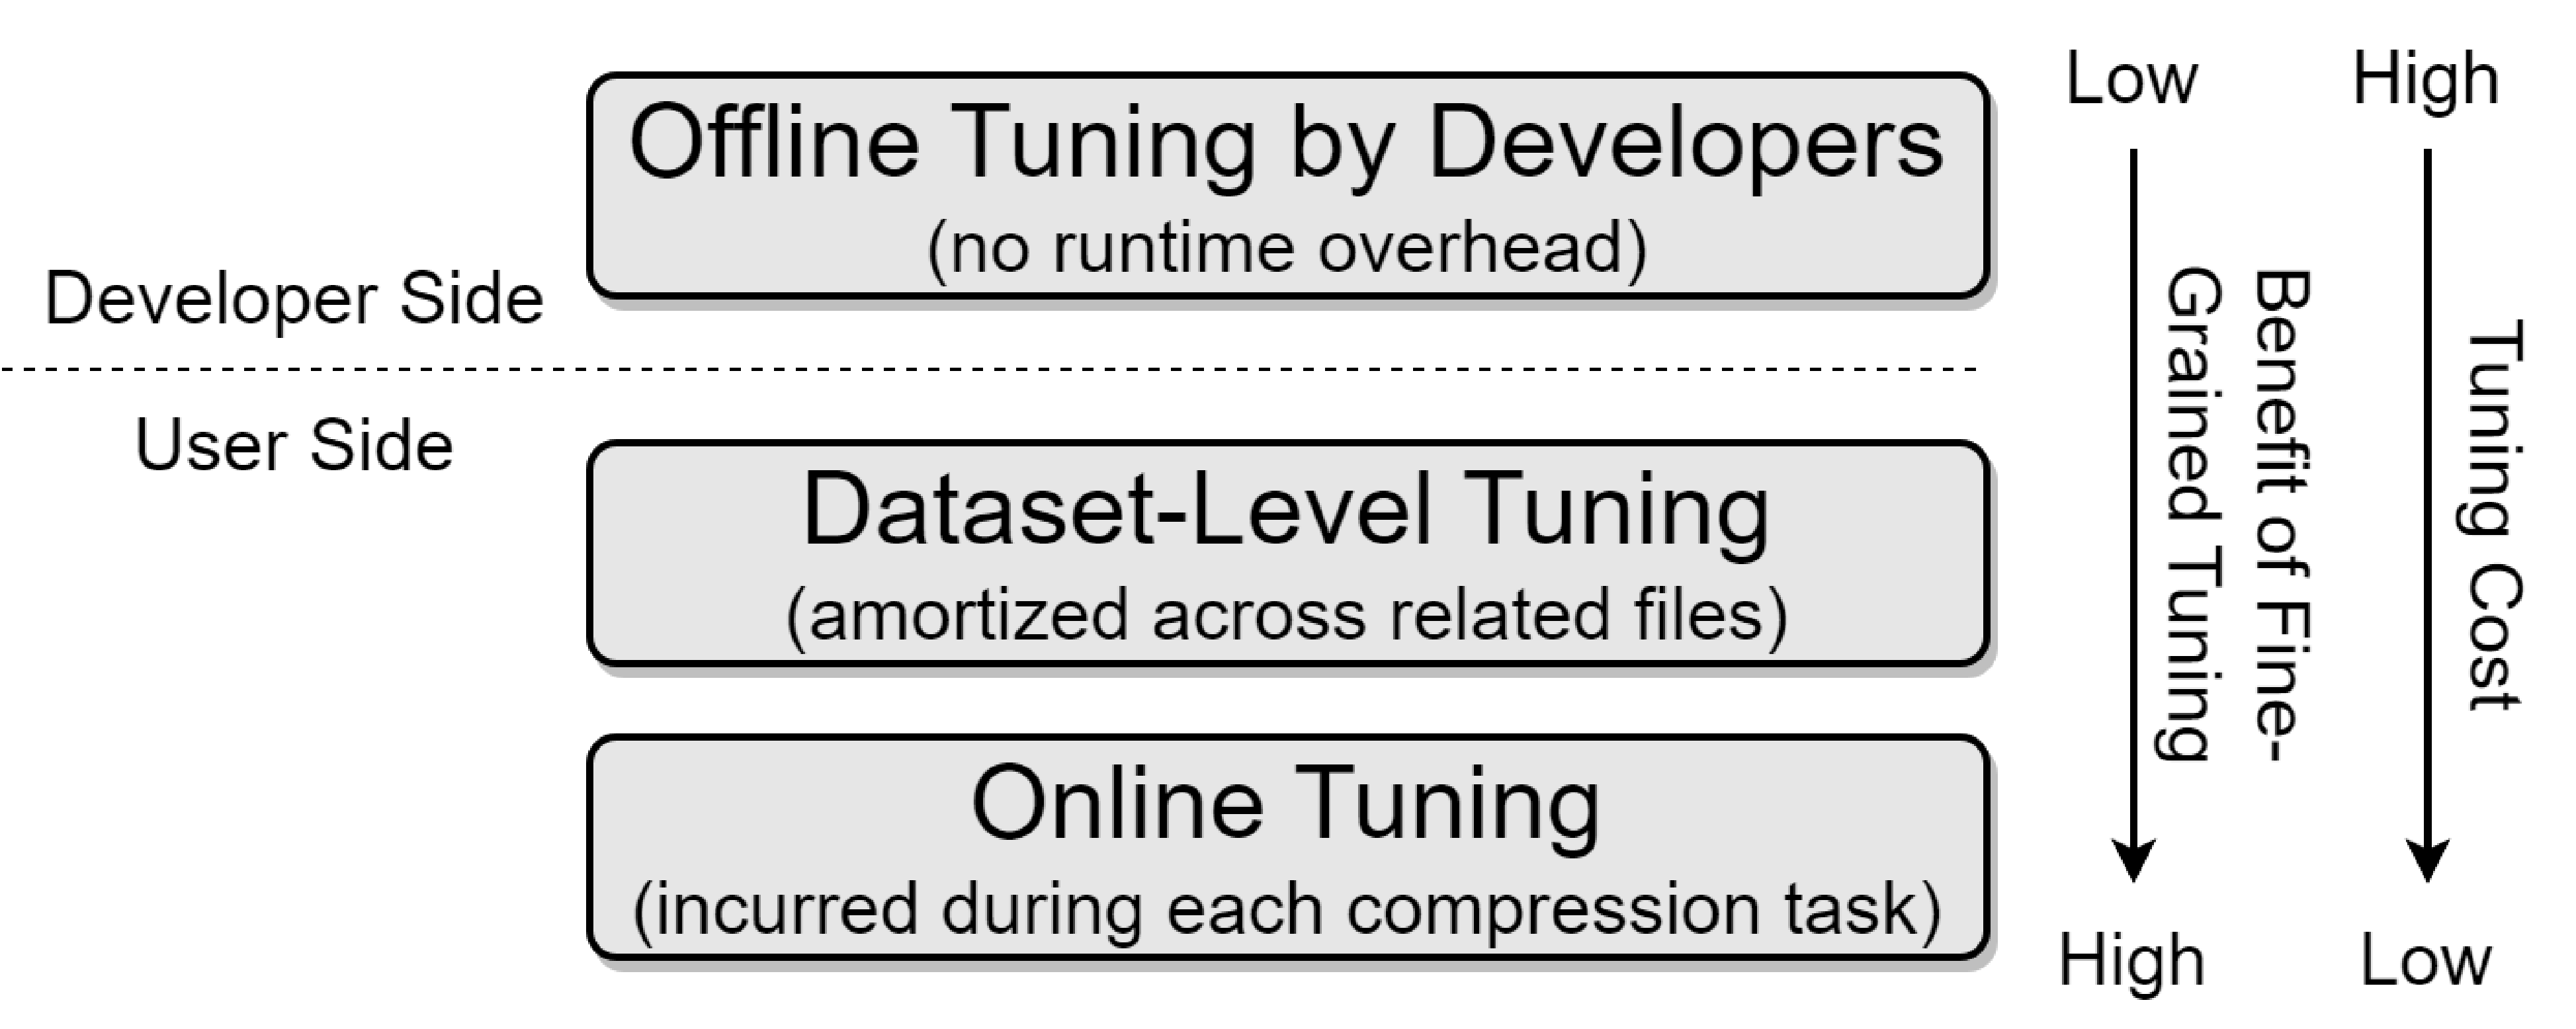
\includegraphics[width=0.7\linewidth]{figs/3/diagram1.pdf}
    \caption{Hierarchical Organization of Configuration Tuning}
    \label{fig:diagram1}
\end{figure}

Exploring all configuration dimensions uniformly at runtime is neither necessary nor practical. As illustrated in Figure~\ref{fig:diagram1}, we therefore assign different tuning steps to three stages: offline tuning performed by compressor developers across multiple datasets, dataset-level tuning performed before compression on representative data, and online tuning performed during compression for individual files or data blocks. Offline tuning introduces no runtime overhead for users, while dataset-level tuning costs can be amortized across related files. In contrast, online tuning costs are incurred during compression and must therefore remain sufficiently low.

The appropriate stage for each configuration dimension depends on its expected benefit and tuning cost. These two aspects are determined by several interrelated factors. We consider the following factors:

\begin{itemize}
\item \textbf{Regularity of the performance landscape} describes how smoothly and predictably compression performance changes as a numerical configuration varies while other configurations are fixed. If the response is smooth and approximately unimodal, a near-optimal value can often be identified using only a small number of evaluations. The regularity of the response may depend on the amount of data used for evaluation. Aggregating performance over an entire dataset or a large data region tends to average out local variations, whereas evaluation on a small data block may produce irregular fluctuations caused by its limited and highly localized data characteristics.

\item \textbf{Magnitude of the potential gain} describes the expected maximum performance improvement achievable through tuning relative to a fixed default choice. Dimensions with limited potential gains may not justify expensive or repeated tuning.

\item \textbf{Generalizability} describes whether a selected configuration can be reused across datasets or across related files, variables, or timesteps. Greater reuse allows the tuning overhead to be amortized over more compression tasks.

\item \textbf{Size of the candidate space} describes the number of possible choices and, consequently, the number of candidates that may need to be evaluated. For categorical or integer-valued configurations, the candidate space is explicitly defined. For continuous-valued configurations, however, its effective size depends on both the search range and the sampling resolution. The required resolution is further influenced by the regularity of the performance landscape and the magnitude of the potential tuning gain.

\item \textbf{Interaction with other configuration dimensions} describes the extent to which the best choice for one dimension depends on the choices made for other dimensions. Weakly interacting dimensions can be tuned independently or sequentially, while strongly interacting dimensions may require joint search.

\item \textbf{Availability and reliability of proxy metrics} describes whether candidate configurations can be evaluated without executing the complete compression pipeline. An inexpensive and sufficiently reliable proxy can enable fine-grained online tuning by reducing the per-candidate evaluation cost. However, a proxy that poorly preserves the relative ranking of candidates may lead to suboptimal decisions, even if it is inexpensive to compute.
\end{itemize}

These factors should be considered jointly rather than as independent assignment rules. Each factor indicates a tendency toward a particular tuning stage, so a configuration dimension may be suitable for more than one stage. The final assignment is therefore necessarily empirical and may involve trade-offs between data-specific adaptation and practical preprocessing and execution overhead.
\section{Tunable Dimensions in the SZ Compression Pipeline}\label{sec:tunable dimensions}

In this section, we first review the general workflow of the SZ compression pipeline. We then identify the tunable configuration dimensions exposed by this pipeline and analyze their potential benefits and tuning costs under the hierarchical framework introduced in Section~\ref{sec:framework}, with the goal of determining appropriate tuning stages for different dimensions.

\subsection{SZ Compression Pipeline}

\begin{figure}[htb]
    \centering
    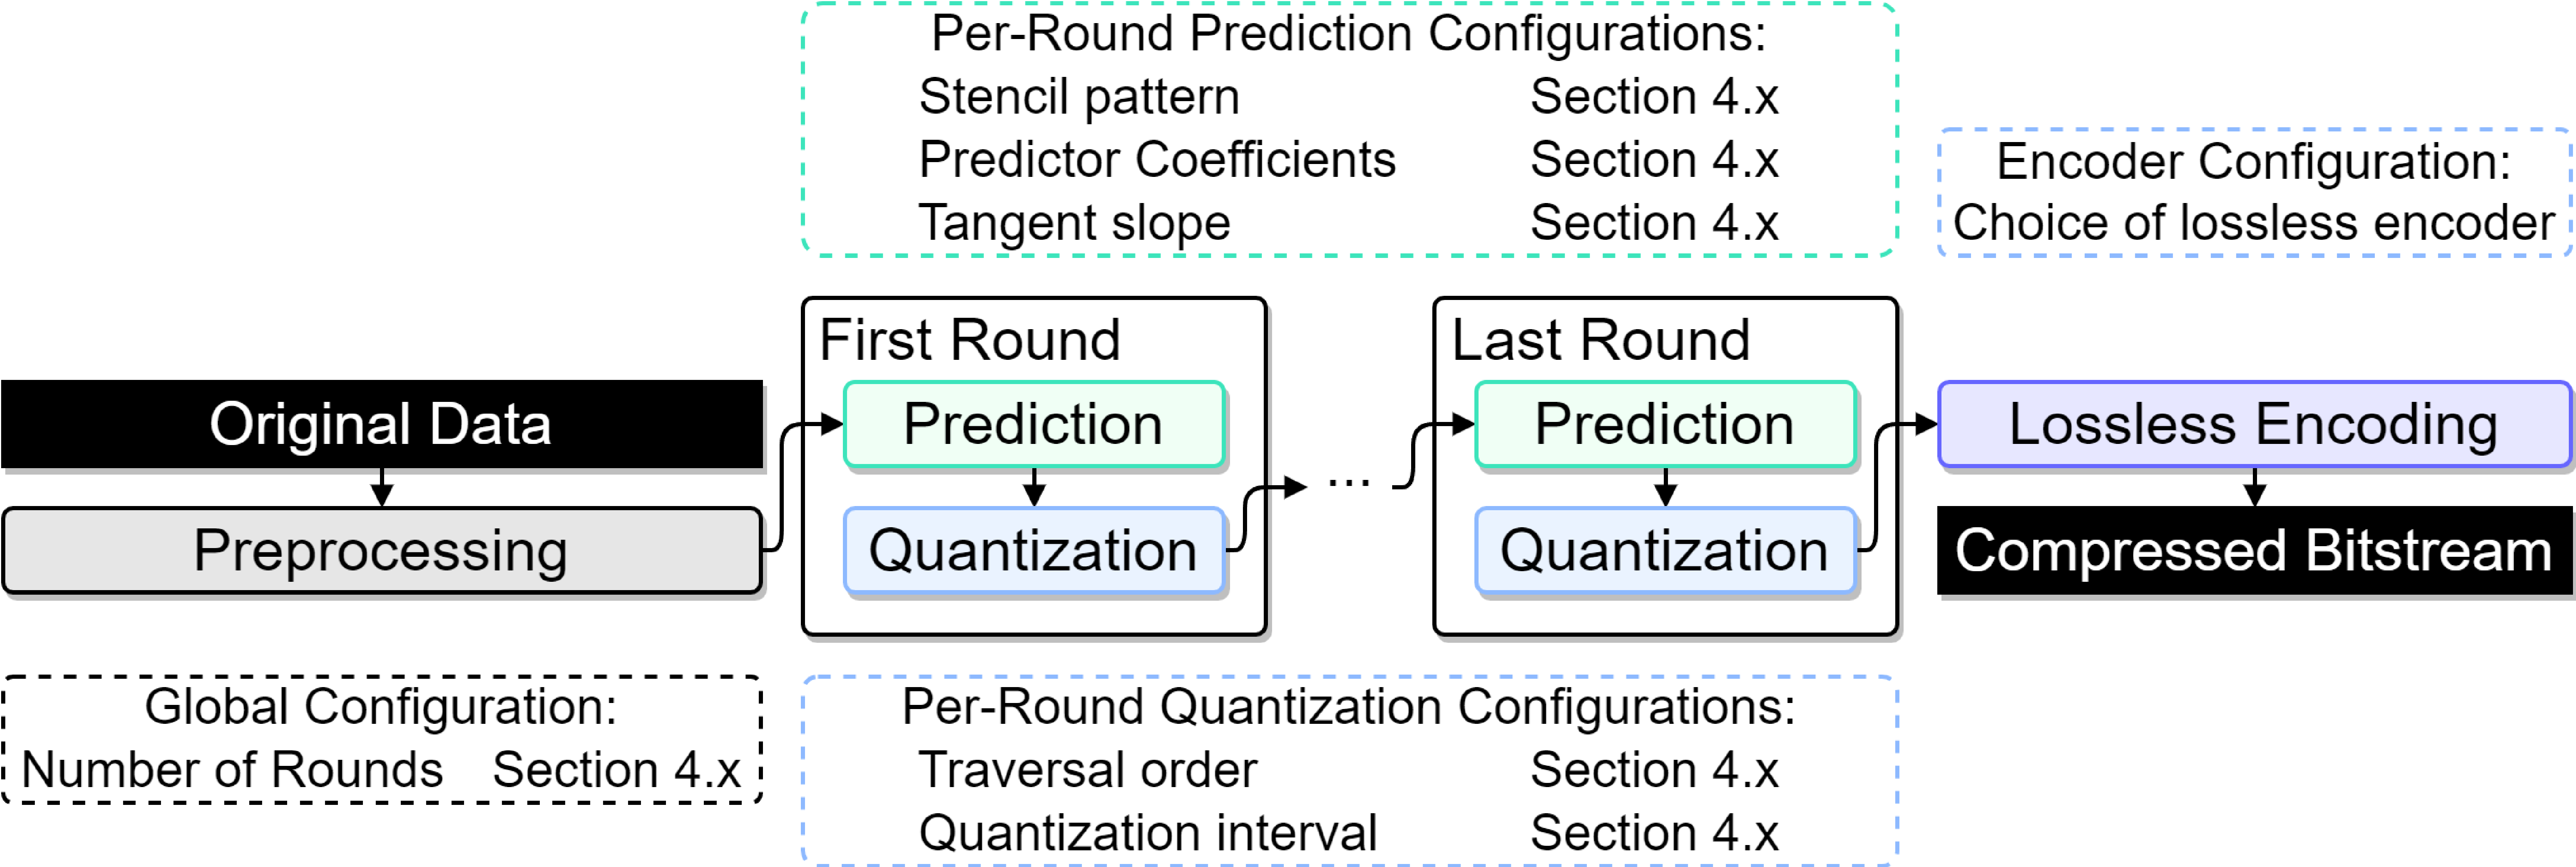
\includegraphics[width=1\linewidth]{figs/4/diagram2.pdf}
    \caption{Enter Caption}
    \label{fig:diagram2}
\end{figure}

The SZ compression pipeline mainly consists of three components: prediction, quantization of prediction residuals, and lossless encoding. As illustrated in Figure~\ref{fig:diagram2}, the prediction and quantization stages are divided into multiple rounds and executed iteratively. Each prediction round reconstructs a new set of data values, which can then serve as references in subsequent rounds. Lossless compression is applied only after the quantized residuals of all prediction rounds have been generated. The three components are described as follows.

\begin{itemize}
\item \textbf{Prediction.} A predictor commonly used in the SZ pipeline computes a weighted sum of selected reconstructed data points, referred to as \emph{reference points}, to estimate a data value that has not yet been reconstructed, referred to as the \emph{prediction target}. During decompression, the original data are unavailable, and the predictor can only access values that have already been reconstructed. Therefore, reference points must be selected exclusively from previously reconstructed data so that the compressor and decompressor can generate identical predictions. Such a weighted-sum predictor is characterized by a \emph{stencil pattern} and a set of \emph{coefficients}. The stencil pattern specifies the relative locations of the reference points with respect to the prediction target. The coefficients specify the weights assigned to the individual reference points.

Prediction is typically organized into multiple rounds. In each round, the number of newly predicted targets is approximately equal to the total number of values already reconstructed. Consequently, later rounds process progressively larger portions of the dataset and therefore have a substantially greater impact on the overall compression performance than earlier rounds.

\item \textbf{Quantization of prediction residuals.} For each prediction target, the compressor computes the difference between its original value and predicted value, and quantizes this residual to an integer multiple of the quantization interval $\Delta$. The quantized residual is then added to the prediction to obtain the reconstructed lossy value.

In the standard setting, choosing $\Delta=2\epsilon$, where $\epsilon$ is the user-specified error bound, guarantees pointwise error boundedness. However, a narrower quantization interval also preserves the error bound.

\item \textbf{Lossless compression.} After all prediction residuals have been quantized, the resulting integer symbols are losslessly encoded. Liu et al.~\cite{liu2021improving} showed that different lossless encoders can lead to different trade-offs between compression ratio and throughput. Their results indicate that Huffman coding followed by Zstandard compression provides moderate compression ratios while achieving the highest compression throughput. We therefore fix this encoding pipeline in ASZ and focus our configuration exploration on prediction and quantization.
\end{itemize}

\subsection{Tangent-Based Rate--Distortion Comparison}\label{sec:tunable dimensions:tangent}

The objective of error-bounded lossy compression is to achieve both a lower bit rate and higher reconstruction quality. However, a configuration change often introduces a trade-off between these two metrics: it may improve PSNR while increasing the bit rate, or reduce the bit rate at the cost of lower PSNR. Prior work by Liang et al.~\cite{liang2019significantly} compares configurations by adjusting their error bounds until they achieve the same bit rate or PSNR. Although this approach enables a direct comparison, it may require multiple additional compression runs.

\begin{figure}[htb]
    \centering
    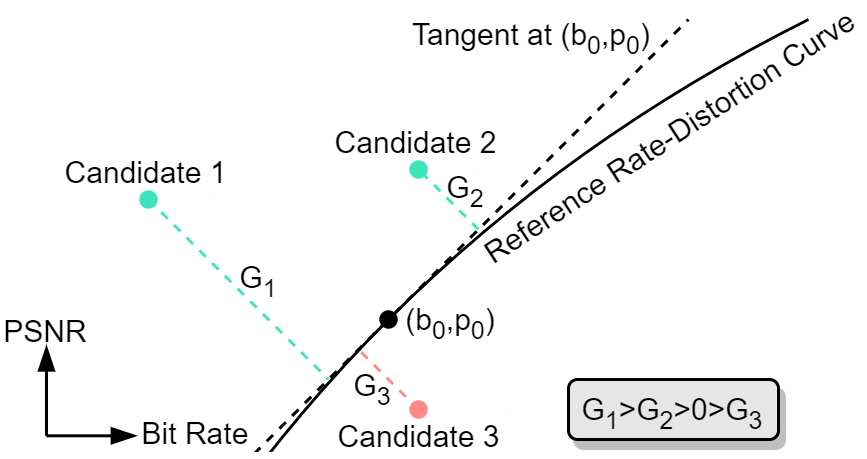
\includegraphics[width=0.7\linewidth]{figs/4/projection.png}
    \caption{Tangent-Based Rate--Distortion Comparison}
    \label{fig:tangent}
\end{figure}

To avoid this additional evaluation overhead, we propose a tangent-based rate--distortion comparison criterion, as illustrated in Figure~\ref{fig:tangent}. Given a reference configuration and a target error bound $eb_0$, we estimate the tangent of its rate--distortion curve at the corresponding operating point $(b_0,p_0)$, where $b_0$ denotes the bit rate and $p_0$ denotes PSNR. Specifically, we evaluate the reference configuration at two nearby error bounds on opposite sides of $eb_0$, namely, $eb_{\mathrm{low}}=eb_0/r$ and $eb_{\mathrm{high}}=eb_0r$, where $r>1$, obtaining the corresponding operating points $(b_{\mathrm{low}},p_{\mathrm{low}})$ and $(b_{\mathrm{high}},p_{\mathrm{high}})$. We approximate the local rate--distortion slope as
\begin{equation}
m_{\mathrm{RD}}=\frac{p_{\mathrm{high}}-p_{\mathrm{low}}}{b_{\mathrm{high}}-b_{\mathrm{low}}}.
\end{equation}

The estimated tangent at $(b_0,p_0)$ is expressed as
\begin{equation}
p-p_0=m_{\mathrm{RD}}(b-b_0).
\end{equation}

For a candidate configuration with operating point $(b_c,p_c)$ under the same error bound $eb_0$, we define its gain as the normalized signed offset from $(b_c,p_c)$ to the reference tangent:
\begin{equation}
G=\frac{p_c-p_0-m_{\mathrm{RD}}(b_c-b_0)}{\sqrt{1+m_{\mathrm{RD}}^2}}.
\end{equation}

A positive value of $G$ indicates that the candidate lies above the reference tangent, toward the preferred upper-left region of the rate--distortion plane, and therefore improves the local rate--distortion trade-off. $G=0$ indicates that the candidate moves only along the local rate--distortion trend. Therefore, candidates with larger values of $G$ are preferred.

\subsection{Analysis of Tunable Configuration Dimensions}\label{sec:tunable dimensions:analysis}

In the remainder of this section, we provide a more detailed explanation of the tunable configuration dimensions summarized in Figure~\ref{fig:diagram2}. For each dimension, we analyze its potential rate--distortion benefit, tuning costs and generalizability. Based on these factors, we determine the appropriate tuning stage within the hierarchical framework shown in Figure~\ref{fig:diagram1}. We first examine stencil patterns and predictor coefficients in Sections~\ref{sec:tunable dimensions:analysis:TC predictor}---~\ref{sec:tunable dimensions:analysis:coefficients},as these two dimensions are closely coupled and jointly determine the behavior of a predictor. We then analyze XXX.

\subsubsection{Tunable-Coefficient Predictors}\label{sec:tunable dimensions:analysis:TC predictor}\mbox{}

A weighted-sum predictor is jointly characterized by its stencil pattern and coefficients. The stencil pattern specifies the locations of the reference points relative to the prediction target, while the coefficients determine how these references are combined. In principle, a predictor may use reference points from a large neighborhood to exploit more information. In practice, however, only previously reconstructed values are available to both compression and decompression, and larger stencils increase computation costs. The stencil pattern therefore determines a restricted set of usable references.

\begin{figure}[htb]
    \centering
    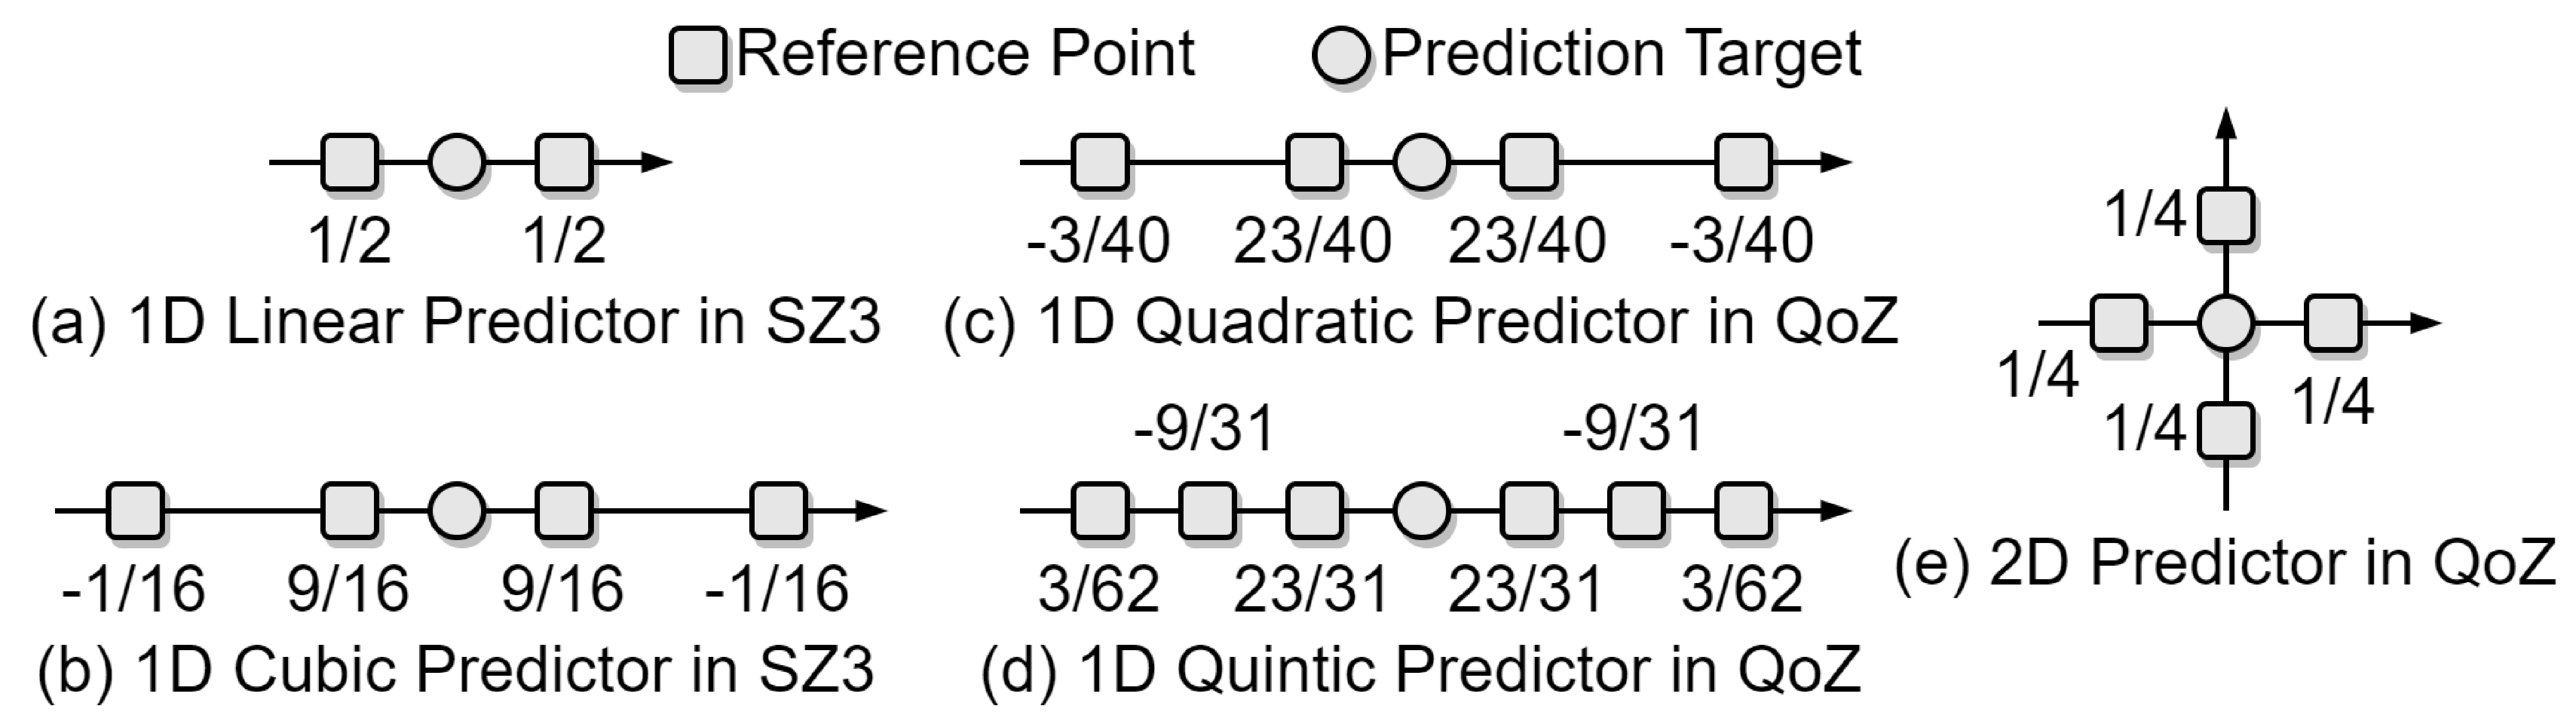
\includegraphics[width=1\linewidth]{figs/4/stencil patterns.pdf}
    \caption{Enter Caption}
    \label{fig:sp}
\end{figure}

Figure~\ref{fig:sp} illustrates several predictors used in SZ3 and QoZ. Additional predictors can be obtained by rotating these stencil patterns to align with different spatial dimensions. 

Both compressors include a predictor with four reference points along the same line (1D cubic predictor in SZ3 and 1D quadratic predictor in QoZ). However, they assign different coefficients to the same stencil pattern because they make different assumptions about local data behavior. SZ3 derives its coefficients by fitting a cubic polynomial through the four reference points, whereas QoZ constructs a piecewise quadratic spline under zero-slope boundary conditions. Other assumptions about local data characteristics can lead to different coefficient assignments. For example, under a stationary AR(1) correlation model, as the correlation parameter increases from $0$ toward $1$, the MSE-optimal coefficient assigned to each of the two reference points nearest to the prediction target increases from $0.25$ toward $0.5$. Meanwhile, the coefficients of the two outer reference points decrease from $0.25$ toward $0$. Notably, the coefficients assigned to the two inner reference points by SZ3 and QoZ are both greater than $0.5$, and therefore cannot be obtained under this stationary AR(1) model for any correlation parameter in $[0,1)$. These examples indicate that different assumptions about local data behavior lead to substantially different coefficient assignments, and no fixed coefficient assignment is uniformly optimal across different data characteristics.

Motivated by this observation, we define a ``tunable-coefficient predictor'' as a predictor with a fixed stencil pattern but adjustable coefficients. We constrain the coefficients to sum to one so that the prediction is exact for constant-valued data. Since all stencil patterns considered in this work are symmetric, coefficients at symmetric reference locations are constrained to be equal. When evaluating a tunable-coefficient predictor, we uniformly sample the feasible coefficient space and report the coefficient assignment that performs best under the tangent-based rate--distortion criterion introduced in Section~\ref{sec:tunable dimensions:tangent}.

\begin{figure}
    \centering
    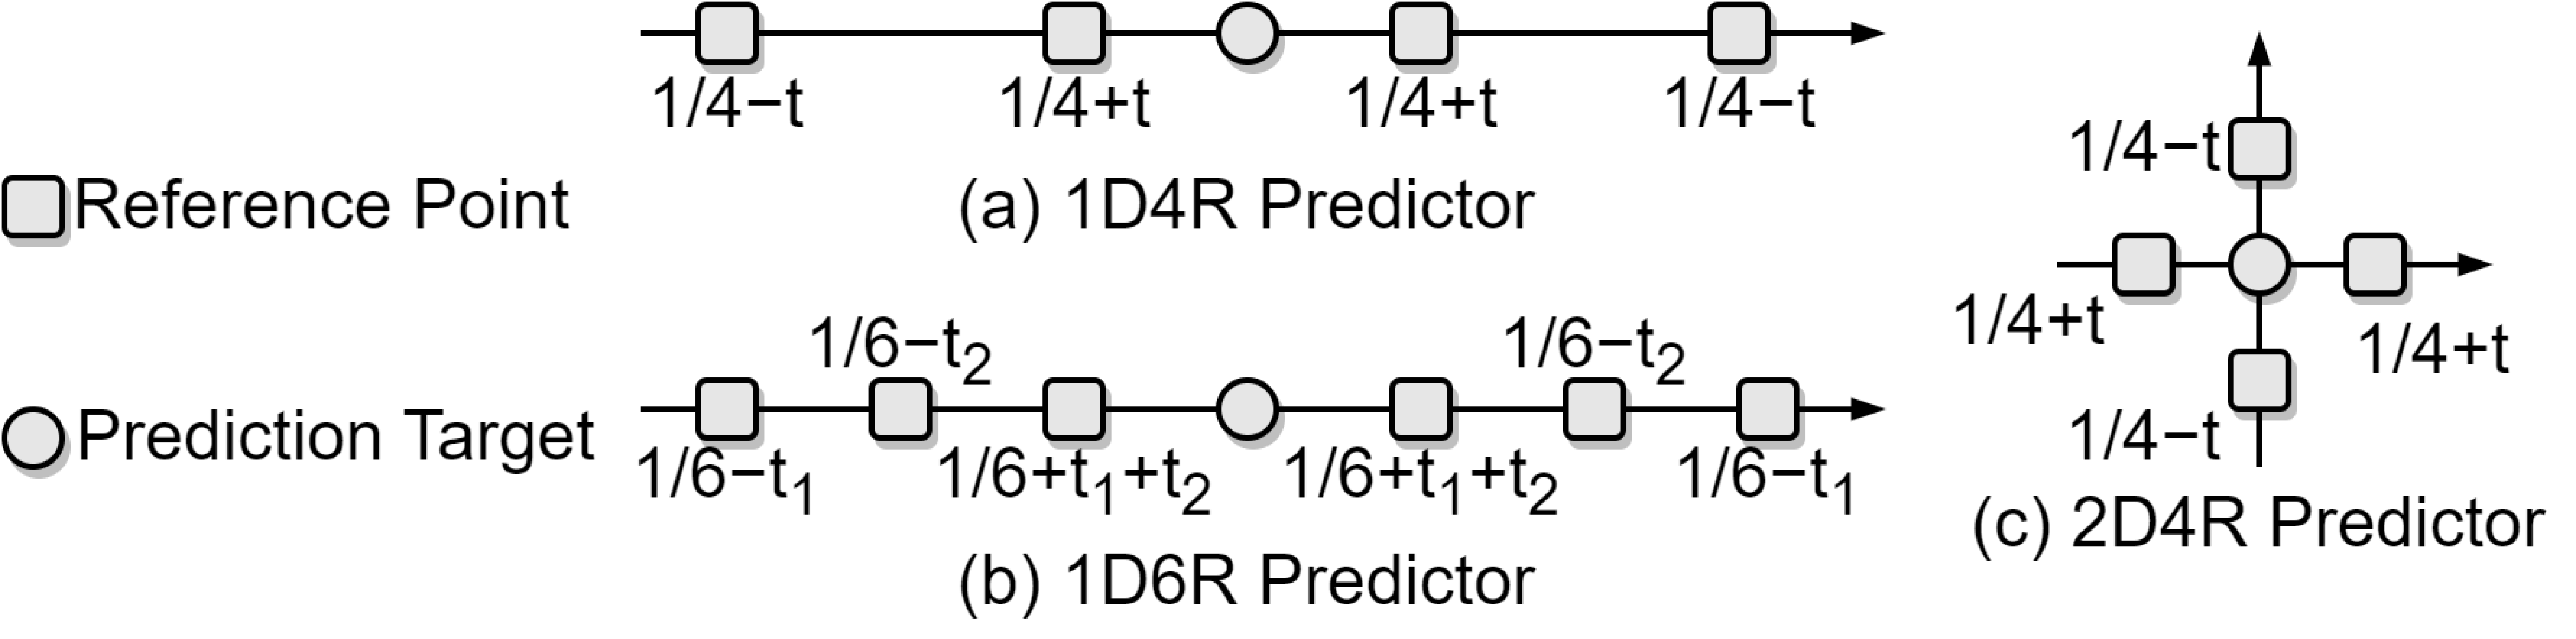
\includegraphics[width=1\linewidth]{figs/4/tunable coefficient stencil patterns.pdf}
    \caption{Enter Caption}
    \label{fig:tcsp}
\end{figure}

Predictors obtained by orienting the stencil geometry along different spatial directions form a predictor family. Figure~\ref{fig:tcsp} illustrates the three tunable-coefficient predictor families considered in this work. We use the notation $X$D$Y$R to denote a family whose predictors use $Y$ reference points distributed across $X$ spatial dimensions. 1D4R predictor family generalizes the linear and cubic predictors in SZ3 and the quadratic predictor in QoZ. Similarly, the 2D4R family generalizes the 2D predictor in QoZ, while the 1D6R family generalizes the quintic predictor in QoZ.

We evaluate the three tunable-coefficient predictor families on the ISABEL and CLDICE datasets in Table~\ref{tab:datasets}, and report their rate--distortion performance in Figure~\ref{fig:compare sp}. Both datasets are three-dimensional. Therefore, each predictor family can be instantiated along three orientations, corresponding to the three curves of the same color. The results lead to two main observations.

\begin{figure}[htb]
    \centering
    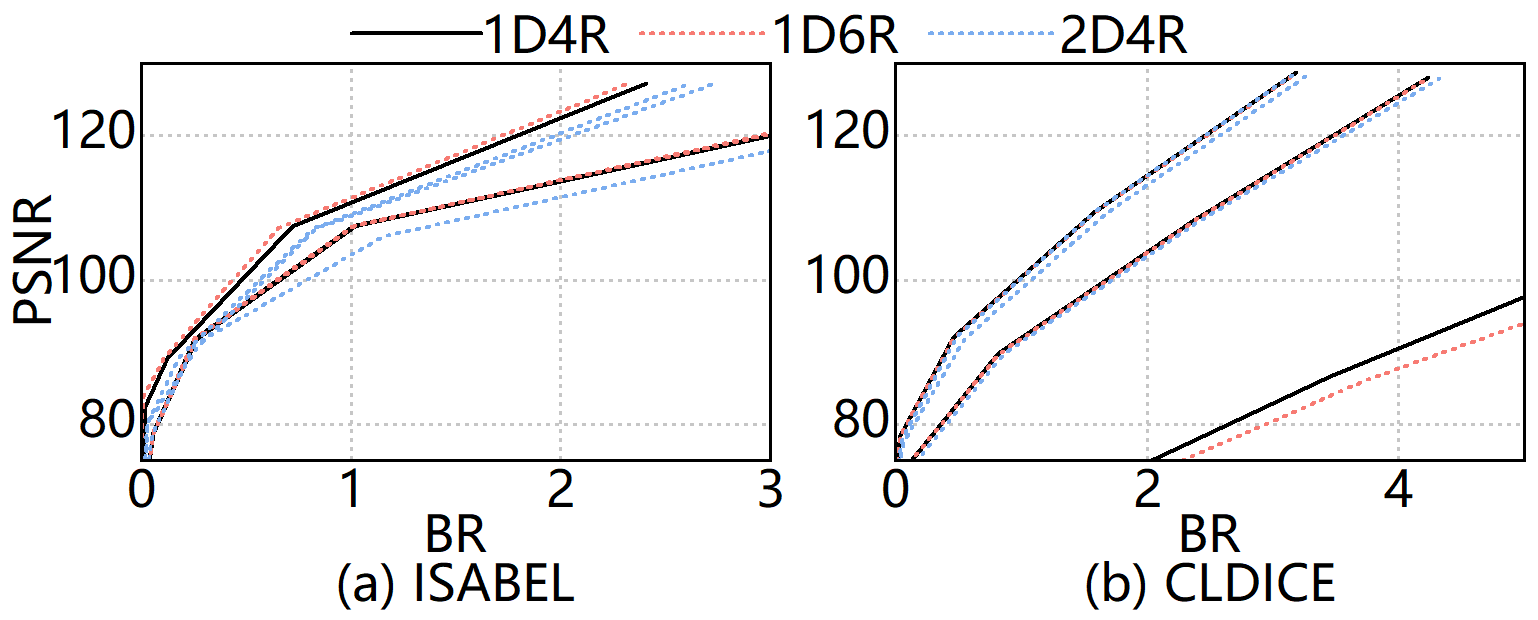
\includegraphics[width=0.8\linewidth]{figs/4/比较stencil pattern.png}
    \caption{Enter Caption}
    \label{fig:compare sp}
\end{figure}

\begin{itemize}
\item \textbf{The 2D4R predictors consistently underperform the 1D4R predictors.} After coefficient tuning, a 1D4R predictor can adaptively determine how much local nonlinear variation around the prediction target should be exploited. On noisy data, this information is often unreliable, and the optimal coefficients tend to approach those of the linear predictor in SZ3. On smoother data, the optimal coefficients tend to move toward those of the cubic predictor in SZ3 or the quadratic predictor in QoZ. This behavior suggests that the preferred 1D4R coefficients primarily reflect the overall usefulness of local nonlinear information, which is strongly influenced by the noise level and is often relatively consistent across a dataset.

In contrast, a 2D4R predictor can be viewed as a weighted combination of two one-dimensional linear predictions along different dimensions. Since neither component captures local nonlinear information, the resulting prediction errors contain unresolved nonlinear components from both directions. Appropriate coefficients may partially cancel these errors, but such cancellation is highly dependent on local data behavior and therefore does not generalize well across the dataset. This provides a possible explanation for the consistently weaker performance of 2D4R predictors.

\item \textbf{The improvement of 1D6R over 1D4R is very limited.} As shown in Figure~\ref{fig:compare sp}, the difference between the best 1D6R and 1D4R predictors is substantially smaller than the difference between the three oriented 1D4R predictors. Moreover, 1D6R introduces a larger coefficient-search space and incurs slightly higher prediction cost because it uses more reference points. We therefore exclude both 2D4R and 1D6R from the subsequent tuning space and retain 1D4R as the tunable-coefficient predictor family used in ASZ.
% 补充一下1D4R的参数搜索空间其实是1D6R的子集，所以最好的1D6R一定比最好的1D4R更好，但是优势非常少。
\end{itemize}

\subsubsection{Tuning Sequence of Stencil Patterns}\mbox{}

Existing compressors have explored tuning stencil patterns across prediction rounds, but only within restricted sequence structures. For three-dimensional data, SZ3 organizes every three consecutive rounds into a group, with the three rounds performing one-dimensional prediction along the three spatial dimensions, respectively. The prediction directions can be reordered within a group, but the same order is reused across all groups. QoZ expands this design by introducing two-dimensional predictors and allowing different groups to use different prediction orders. Nevertheless, both approaches retain the group structure and therefore explore only a restricted subset of possible prediction sequences.

We remove this grouping constraint and allow the differently oriented 1D4R predictors to be arranged freely across prediction rounds. The resulting search space grows exponentially with the number of rounds, making exhaustive evaluation impractical. We therefore adopt a backward greedy strategy that prioritizes the later prediction rounds. Specifically, we first select the stencil pattern for the final round and then proceed backward through the preceding rounds. Later rounds process substantially more prediction targets than earlier rounds and therefore generally have a greater impact on the overall rate--distortion performance. By fixing these high-impact choices first, the backward search provides an efficient approximation to exhaustive sequence tuning.

\begin{figure}[htb]
    \centering
    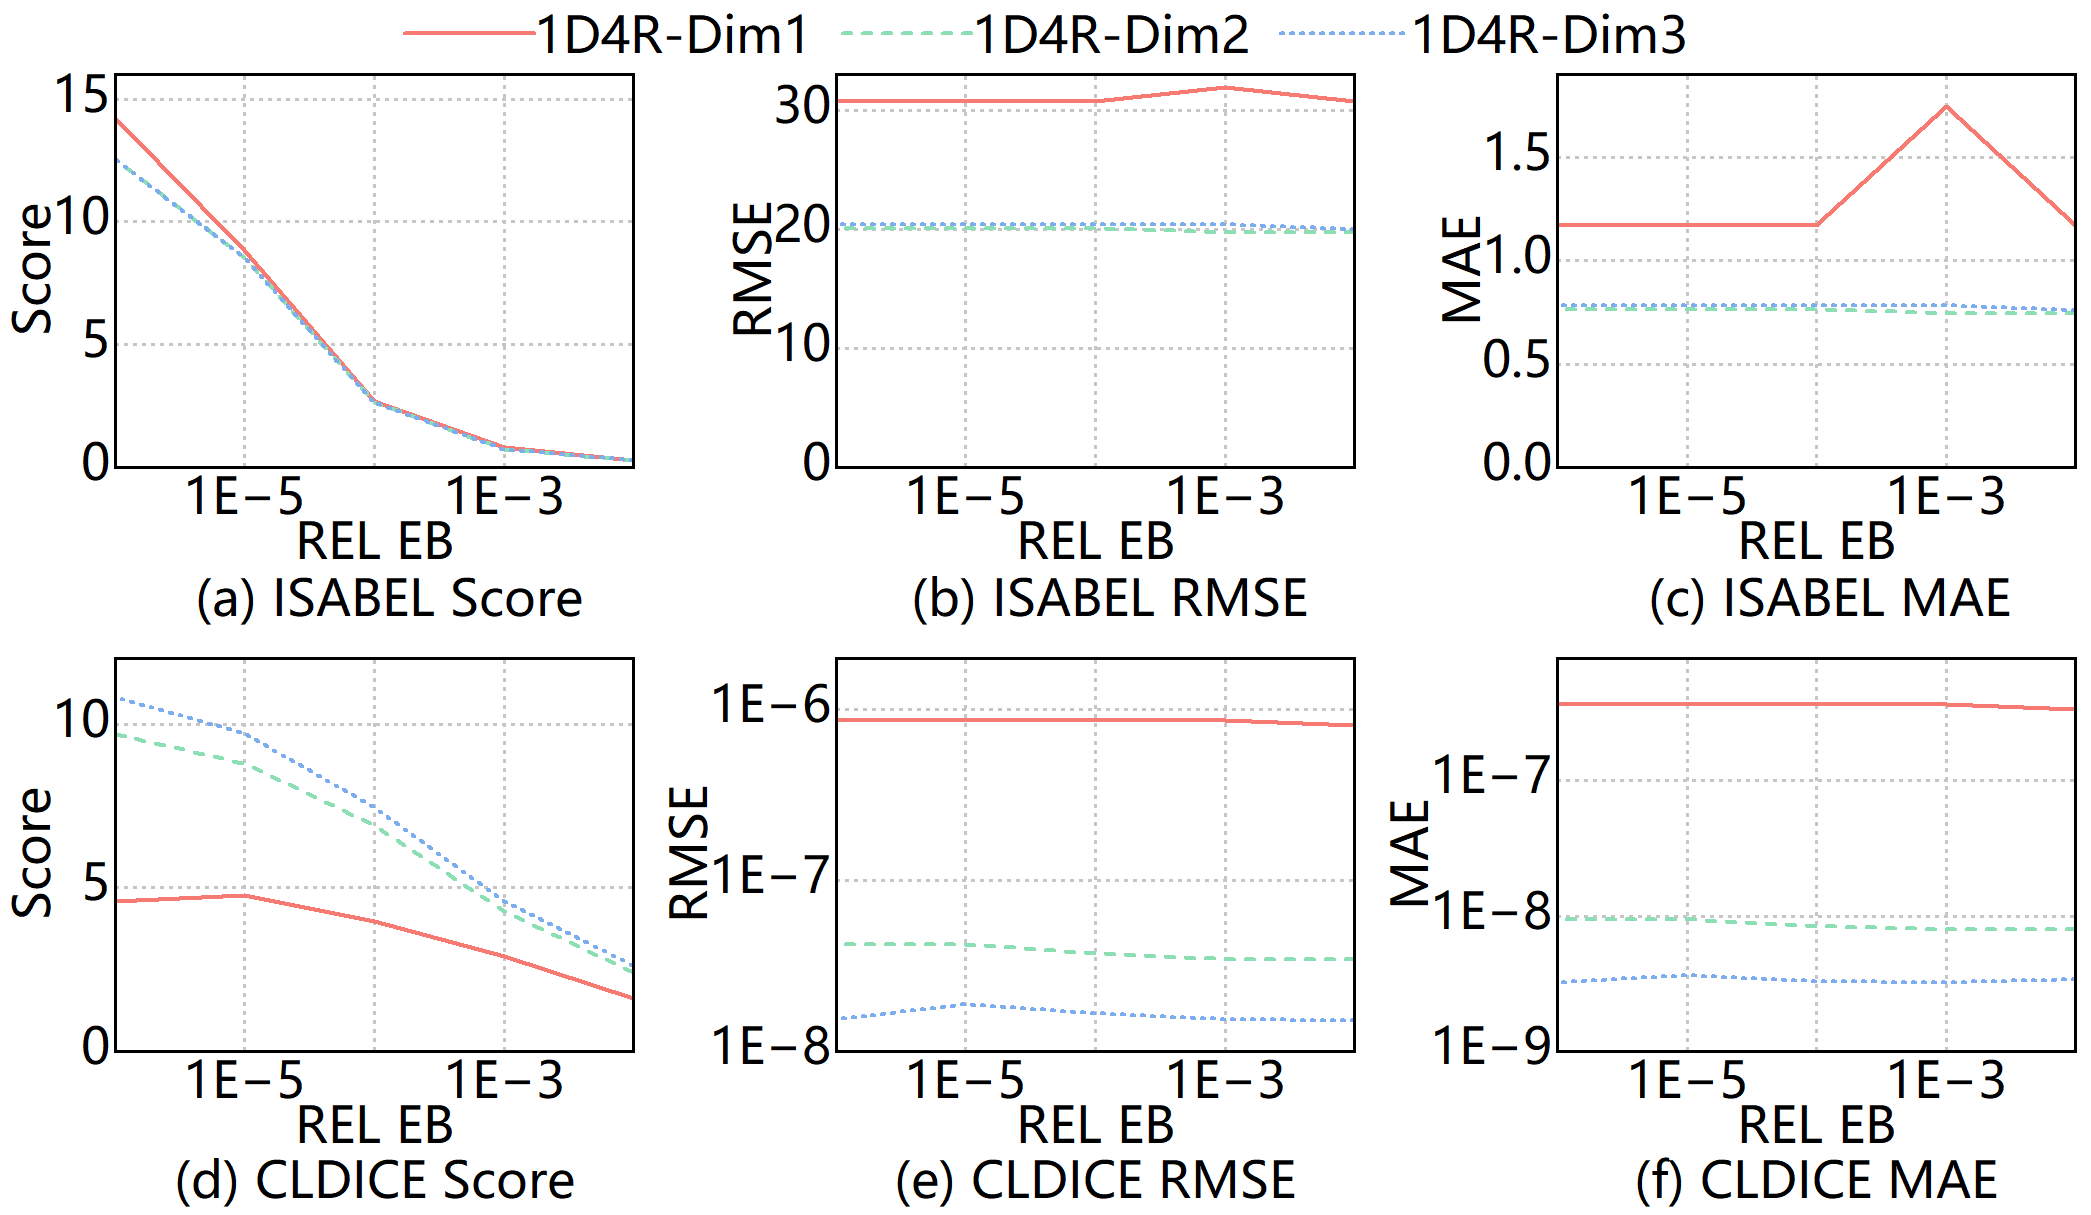
\includegraphics[width=1\linewidth]{figs/4/检验stencil pattern的proxy.png}
    \caption{Enter Caption}
    \label{fig:verify sp proxy}
\end{figure}

By comparing the solid black curves in Figure~\ref{fig:compare sp}, we observe that tuning the stencil pattern can provide significant rate--distortion improvement. However, we do not identify a reliable proxy for accelerating this tuning process.
Figure~\ref{fig:verify sp proxy} compares the tangent-based bit-rate--PSNR scores, prediction RMSE, and prediction MAE of the 1D4R predictors oriented along the three spatial dimensions on the ISABEL and CLDICE datasets. In principle, a well-performing predictor is expected to achieve a high rate--distortion score together with low prediction RMSE and MAE. However, this relationship is not consistently observed. On ISABEL, the predictor oriented along the first dimension achieves a high rate--distortion score despite also exhibiting high RMSE and MAE. Consequently, neither RMSE nor MAE reliably preserves the ranking of stencil candidates and therefore cannot serve as an effective proxy for stencil-pattern tuning. We further discuss the cause of this discrepancy in Section~\ref{sec:discussion}.

% 还要验证跨文件普适性

\subsubsection{Tuning Coefficients}\label{sec:tunable dimensions:analysis:coefficients}\mbox{}

After selecting a 1D4R predictor, we further examine whether tuning its coefficients provides meaningful rate--distortion improvement. On the ISABEL and CLDICE datasets, we apply the best-performing 1D4R predictor identified in the preceding analysis and vary only its coefficient assignment. Figure~\ref{fig:bbb} compares the resulting rate--distortion curves.

The results show that different coefficient assignments can lead to substantial differences in rate--distortion performance. Moreover, the best-performing coefficients vary across datasets and error bounds, confirming that no single fixed assignment consistently achieves the best performance.

Predictor coefficients interact strongly with stencil patterns. Within the 1D4R family, predictors oriented along different dimensions may favor different coefficient assignments because the data can exhibit different characteristics along these dimensions. Therefore, when tuning stencil patterns, we must first identify the best coefficient assignment for each stencil candidate before comparing their rate--distortion performance. Since this process requires repeated evaluation of coefficient candidates, reducing the cost of each evaluation is essential for efficient stencil-pattern tuning.

\begin{figure}[htb]
    \centering
    \IfFileExists{bbb.pdf}{\includegraphics[width=0.8\linewidth]{bbb.pdf}}{\fbox{\parbox{0.75\linewidth}{\centering Placeholder: coefficient-tuning comparison figure (source file \texttt{bbb.pdf} is missing from the previous manuscript).}}}
    \caption{bbb}
    \label{fig:bbb}
\end{figure}

To reduce this cost, we replace the tangent-based bit-rate--PSNR comparison introduced in Section~\ref{sec:tunable dimensions:tangent} with an $H_1$--PSNR comparison when ranking coefficient assignments for the same stencil predictor. Here, $H_1$ denotes the first-order entropy of the quantized prediction residuals and serves as an estimate of the bit rate. As shown in the first two columns of Figure~\ref{fig:bbb}, replacing bit rate with $H_1$ largely preserves the relative positions of the curves produced by different coefficient assignments, indicating that the $H_1$--PSNR comparison approximates the ranking obtained by the bit-rate--PSNR comparison.

The third column of Figure~\ref{fig:bbb} compares the ranking accuracy of five inexpensive evaluation criteria: the proposed $H_1$--PSNR criterion, $H_1$ alone, PSNR alone, prediction MSE, and prediction MAE. The horizontal axis shows the relative error bound, while the vertical axis reports Kendall's $\tau$ between the candidate ranking produced by each criterion and the ranking produced by the bit-rate--PSNR criterion. Across the evaluated error bounds, the $H_1$--PSNR criterion achieves the highest ranking accuracy.

Compared with the original bit-rate--PSNR criterion, the $H_1$--PSNR criterion first reduces the evaluation cost by eliminating lossless encoding. Both $H_1$ and PSNR can be obtained while computing the quantized prediction errors: $H_1$ is calculated from the resulting symbol distribution, while PSNR is derived from the corresponding reconstruction errors.

A direct evaluation of the $H_1$--PSNR criterion processes each coefficient candidate independently. For each candidate, it predicts all sampled target values, quantizes the resulting prediction errors, counts the frequencies of the quantization symbols to compute $H_1$, and accumulates the reconstruction errors to compute PSNR. Although this approach avoids the lossless-encoding stage required by the bit-rate--PSNR criterion, it still requires prediction and quantization for every combination of coefficient candidate and sampled target.

The evaluation can be further accelerated without explicitly computing and quantizing the prediction error of every sampled target for every coefficient candidate. Both $H_1$ and PSNR depend only on the distribution of prediction errors, rather than on their spatial ordering. Therefore, once an accurate approximation of this distribution is available, the frequencies of the quantized prediction-error symbols and the resulting PSNR can be estimated directly using the following equations.

Let the prediction error $E$ follow a probability density function $f_E(e)$, and let $\Delta$ denote the quantization step size. Under uniform quantization, the probability of quantization symbol $i$ is
\begin{equation}
p_i=\int_{\left(i-\frac{1}{2}\right)\Delta}^{\left(i+\frac{1}{2}\right)\Delta}f_E(e)\,de.
\end{equation}
The first-order entropy is then computed as
\begin{equation}
H_1=-\sum_i p_i\log_2p_i.
\end{equation}
Because an error in the $i$th interval is reconstructed as $i\Delta$, the resulting mean squared reconstruction error is
\begin{equation}
\mathrm{MSE}_{\mathrm{rec}}=\sum_{i=-\infty}^{\infty}\int_{\left(i-\frac{1}{2}\right)\Delta}^{\left(i+\frac{1}{2}\right)\Delta}f_E(e)\left(e-i\Delta\right)^2\,de.
\end{equation}
The corresponding PSNR is
\begin{equation}
\mathrm{PSNR}=10\log_{10}\left(\frac{R^2}{\mathrm{MSE}_{\mathrm{rec}}}\right),
\end{equation}
where $R$ is the value range of the original data.


To efficiently derive the prediction-error distribution,we exploit this property by expressing the prediction error as an affine function of the tunable coefficient. For the 1D4R predictor shown in Figure~\ref{fig:tcsp},the prediction error for a target $x_0$ can be written as
\begin{equation}
\begin{aligned}
e(t)&=x_0-\left[\left(\frac{1}{4}-t\right)x_{-3}+\left(\frac{1}{4}+t\right)x_{-1}\right.\\
&\quad\left.+\left(\frac{1}{4}+t\right)x_1+\left(\frac{1}{4}-t\right)x_3\right]\\
&=At+B,
\end{aligned}
\end{equation}
where
\begin{equation}
A=x_{-3}-x_{-1}-x_1+x_3
\end{equation}
and
\begin{equation}
B=x_0-\frac{x_{-3}+x_{-1}+x_1+x_3}{4}.
\end{equation}

The values of $A$ and $B$ are independent of the coefficient candidate $t$. We therefore compute them once for all sampled prediction targets and construct an approximate joint histogram of $(A,B)$. For a candidate $t$, each occupied histogram bin centered at $(a_j,b_j)$ is mapped to the prediction error $a_jt+b_j$. After quantizing these errors under the target error bound and aggregating the corresponding bin frequencies, we directly obtain an approximation of the quantized-error distribution used to compute $H_1$ and PSNR. This avoids recomputing the prediction error separately for every sampled target and every coefficient candidate.

Let $n$ be the number of sampled prediction targets, $k$ the number of coefficient candidates, and $h$ the number of occupied bins in the joint histogram of $(A,B)$. Direct evaluation computes an error for every target--candidate pair and therefore requires $O(kn)$ time. The histogram-based method requires $O(n)$ time to construct the joint histogram and $O(kh)$ time to evaluate all candidates, resulting in a total complexity of $O(n+kh)$. Since $h$ is typically much smaller than $n$, the evaluation cost is close to linear in the sample size.

The joint histogram need not preserve $A$ and $B$ at full numerical precision. The final $H_1$ calculation only distinguishes prediction errors after quantization, whose interval is determined by the error bound. Therefore, the discretization intervals used for $A$ and $B$ can be substantially smaller than, but need not be comparable to machine precision relative to, the final prediction-error quantization interval. In our implementation, setting their induced error uncertainty to a small fraction of the final quantization interval, such as $10\%$, is sufficient to preserve an accurate quantized-error distribution.

Moreover, the expressions for $A$ and $B$ represent local differences and interpolation residuals, respectively, and are therefore typically concentrated near zero for locally correlated scientific data. As a result, only a limited number of joint-histogram bins are occupied in practice, making $h\ll n$ and reducing the overall evaluation cost to approximately $O(n)$ for a fixed set of coefficient candidates.

\section{Design of ASZ}\label{sec:asz}

\subsection{Overview}

\subsection{Offline Design-Space Exploration}

\subsection{Dataset-Level Dependency-Sequence Tuning}

\subsection{Dataset-Level Traversal-Order Tuning}

\subsection{Efficient Block-Level Coefficient Tuning}

\subsection{Overall Algorithm and Complexity}

\section{Performance Evaluation}
\label{sec:evaluation}

We evaluate ASZ in terms of rate--distortion performance, total runtime across error bounds with per-file tuning, and plan reuse across related files.

\subsection{Experimental Setup}
\label{sec:evaluation:setup}

\subsubsection{Evaluation Platform}

We conduct all experiments on Purdue Anvil. Each standard compute node contains two 64-core AMD EPYC 7763 processors and 235~GiB of memory available to jobs. Every codec execution uses one physical CPU core. We compile ASZ with GCC 11.2.0 using \verb|-Ofast -march=native -mavx2 -mfma|.

\subsubsection{Scientific Datasets}

Table~\ref{tab:evaluation-datasets} summarizes the 18 fields used in the rate--distortion and runtime experiments. They span weather and climate data, seismic imaging, fluid dynamics, cosmology, electronic-structure calculations, hydrodynamics, and X-ray experiments. For the plan-transfer experiments in Section~\ref{sec:evaluation:transfer}, we use related time steps or fields from data sources represented in Table~\ref{tab:evaluation-datasets}.

\begin{table*}[htb]
    \centering
    \caption{Scientific fields used in the evaluation.}
    \label{tab:evaluation-datasets}
    \footnotesize
    \setlength{\tabcolsep}{3pt}
    \begin{tabular}{@{}lll lr@{\hspace{0.8em}}|@{\hspace{0.8em}}lll lr@{}}
        \toprule
        \textbf{Dataset} & \textbf{Field} & \textbf{Index} & \textbf{Domain} & \textbf{Size} &
        \textbf{Dataset} & \textbf{Field} & \textbf{Index} & \textbf{Domain} & \textbf{Size} \\
        \midrule
        QMCPACK & Orbital & 144 & Electronic structure & 2.09~MiB & FLASH & Density & 22 & Hydrodynamics & 32.00~MiB \\
        APS & Kaz & -- & X-ray & 62.38~MiB & Isabel & PRECIP & 24 & Weather & 95.37~MiB \\
        Isabel & QGRAUP & 24 & Weather & 95.37~MiB & Miranda & Velocity-$x$ & -- & Fluid & 144.00~MiB \\
        Miranda & Velocity-$z$ & -- & Fluid & 144.00~MiB & RTM Small & -- & 0360 & Seismic & 180.73~MiB \\
        Aramco & -- & 1800 & Seismic & 180.73~MiB & SCALE-LETKF & PRES & -- & Weather & 538.33~MiB \\
        SCALE-LETKF & T & -- & Weather & 538.33~MiB & CESM & VD01 & 31 & Climate & 642.70~MiB \\
        CESM & UU & 31 & Climate & 642.70~MiB & APS CSSI & -- & L0471 & X-ray & 1.35~GiB \\
        Nyx & Baryon density & 632 & Cosmology & 4.00~GiB & Nyx & Temperature & 632 & Cosmology & 4.00~GiB \\
        APSU & -- & 004 & X-ray & 10.78~GiB & APSU & -- & 006 & X-ray & 43.10~GiB \\
        \bottomrule
    \end{tabular}
\end{table*}

\subsubsection{Baselines and Metrics}

We compare ASZ with two groups of scientific lossy compressors. SZ3, QoZ, and ZFP form the high-performance group, covering prediction-based and block-transform methods. SPERR serves as a high-ratio wavelet-based baseline.

\subsection{Rate--Distortion Performance}
\label{sec:evaluation:rd}

Figure~\ref{fig:evaluation-rd} compares the full RD curves. We summarize each comparison over the common PSNR range as a compression-ratio gain. Across the 18 fields, ASZ achieves geometric-mean compression ratios that are $2.48\times$, $2.07\times$, $6.18\times$, and $1.36\times$ those of SZ3, QoZ, ZFP, and SPERR, respectively. ASZ outperforms SZ3, QoZ, and ZFP on all 18 fields and SPERR on 10 fields.

ASZ improves on SZ3 and QoZ by adapting both prediction and lossless coding at finer granularity. Its unrestricted per-round axis choices can repeatedly use the direction that best matches the correlations at the current reference spacings. For 1D4R, ASZ searches a finer coefficient set within each block than QoZ's predefined one-dimensional formulas, allowing closer adaptation to local correlations. ASZ also selects a QB serialization order for every round, placing strongly correlated QBs consecutively before Huffman encoding and Zstd. These choices reduce prediction residuals and make the QB stream more compressible.

SPERR comes closest to ASZ because both methods perform multiscale spatial decorrelation. ASZ's coarse-to-fine interpolation converts the directional correlations selected in each round into prediction residuals. SPERR instead uses a fixed multilevel three-dimensional CDF 9/7 transform that recursively processes all three axes, exploiting spatial coherence across multiple scales and compacting information into wavelet coefficients. However, this shared principle does not give SPERR ASZ's data-dependent adaptation. SPERR uses a fixed transform rather than selecting the prediction axis and coefficients for each round or block. Its pointwise error guarantee also requires a separate stream of corrections for reconstructed values that exceed the error bound. These differences help explain why ASZ attains a $1.36\times$ geometric-mean compression-ratio advantage and outperforms SPERR on 10 of the 18 fields. SPERR's codec time is also higher because it performs the multilevel transform, repeatedly traverses coefficient bit planes, and applies an inverse transform to locate outliers within each large three-dimensional chunk. The \texttt{sperr3d} default used in our experiments sets the preferred chunk size to $256^3$ values. Section~\ref{sec:evaluation:codec-time} quantifies this time difference.

\begin{figure*}[htb]
    \centering
    \IfFileExists{figs/5/rate-distortion-final-eighteen-log.png}{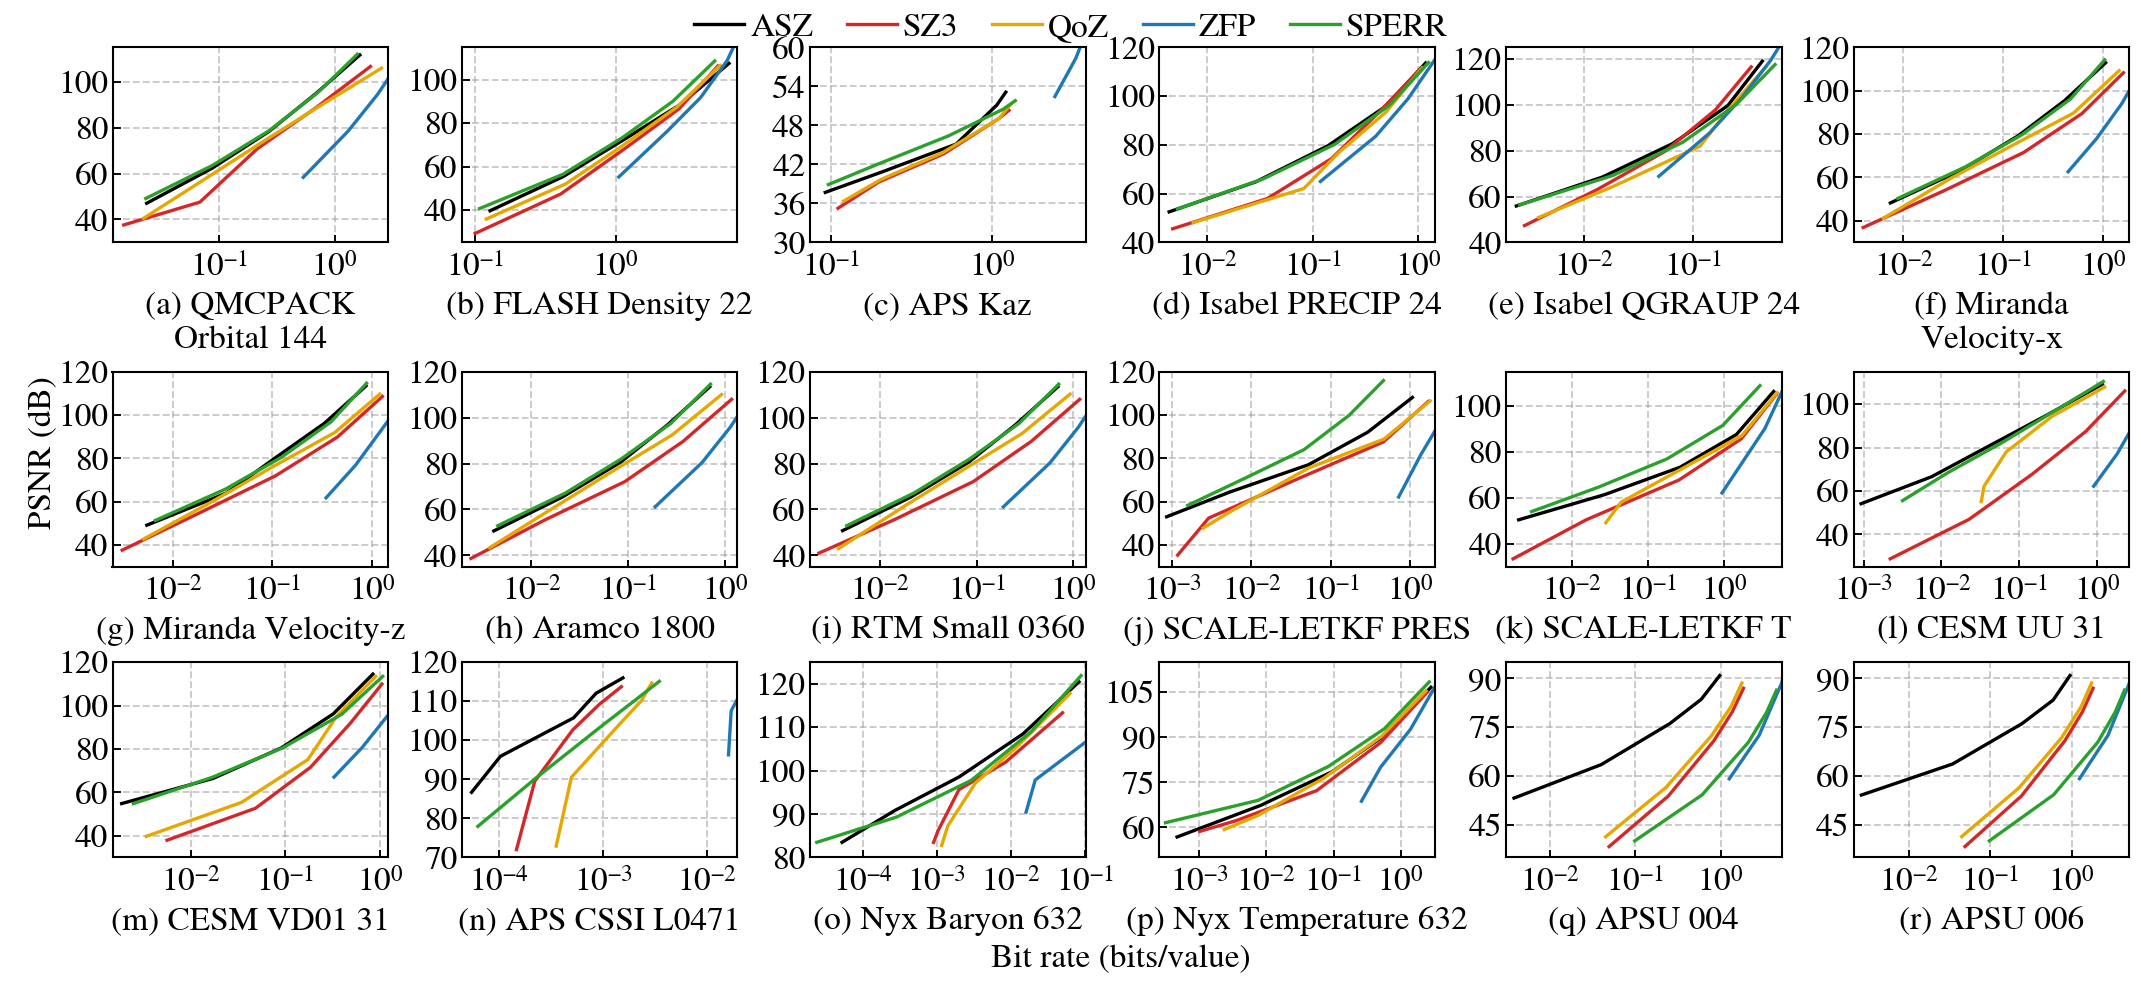
\includegraphics{figs/5/rate-distortion-final-eighteen-log.png}}{\fbox{\parbox[c][1.5in][c]{0.96\textwidth}{\centering Final 18-field rate--distortion figure pending.}}}
    \caption{Rate--distortion performance on 18 scientific fields. At matched PSNR, ASZ achieves $2.48\times$, $2.07\times$, $6.18\times$, and $1.36\times$ the geometric-mean compression ratios of SZ3, QoZ, ZFP, and SPERR, respectively, outperforming the first three on all 18 fields and SPERR on 10.}
    \label{fig:evaluation-rd}
\end{figure*}

\subsection{Total Runtime Across Error Bounds}
\label{sec:evaluation:codec-time}

Figure~\ref{fig:evaluation-codec-time} compares ASZ with SZ3, QoZ, ZFP, and SPERR at all five relative error bounds. Each stacked bar reports the total runtime as the sum of the timed in-memory stages. ASZ includes preprocessing, compression, and decompression, while each baseline includes compression and decompression. File input, file output, and post-run error verification are excluded. ASZ's compression segment includes its data-range scan, and the SZ3 and QoZ compression segments include their built-in tuning. Across the 90 field--error-bound combinations, ASZ's geometric-mean total runtime is $0.81\times$ that of QoZ and $0.43\times$ that of SPERR, and ASZ is faster in 70 and 89 combinations, respectively. Its total runtime is $1.72\times$ that of SZ3 and $2.36\times$ that of ZFP. Considering the timed stages separately, ASZ provides geometric-mean compression and decompression speedups of $1.63\times$ and $1.71\times$ over QoZ and $2.85\times$ and $4.02\times$ over SPERR. At the middle error bound of each field, plan generation accounts for 23.94\% of ASZ's total runtime. These time differences accompany the compression-ratio improvements reported in Section~\ref{sec:evaluation:rd}.

\begin{figure*}[htb]
    \centering
    \IfFileExists{figs/5/time-breakdown-final-eighteen-vs-rel-eb.png}{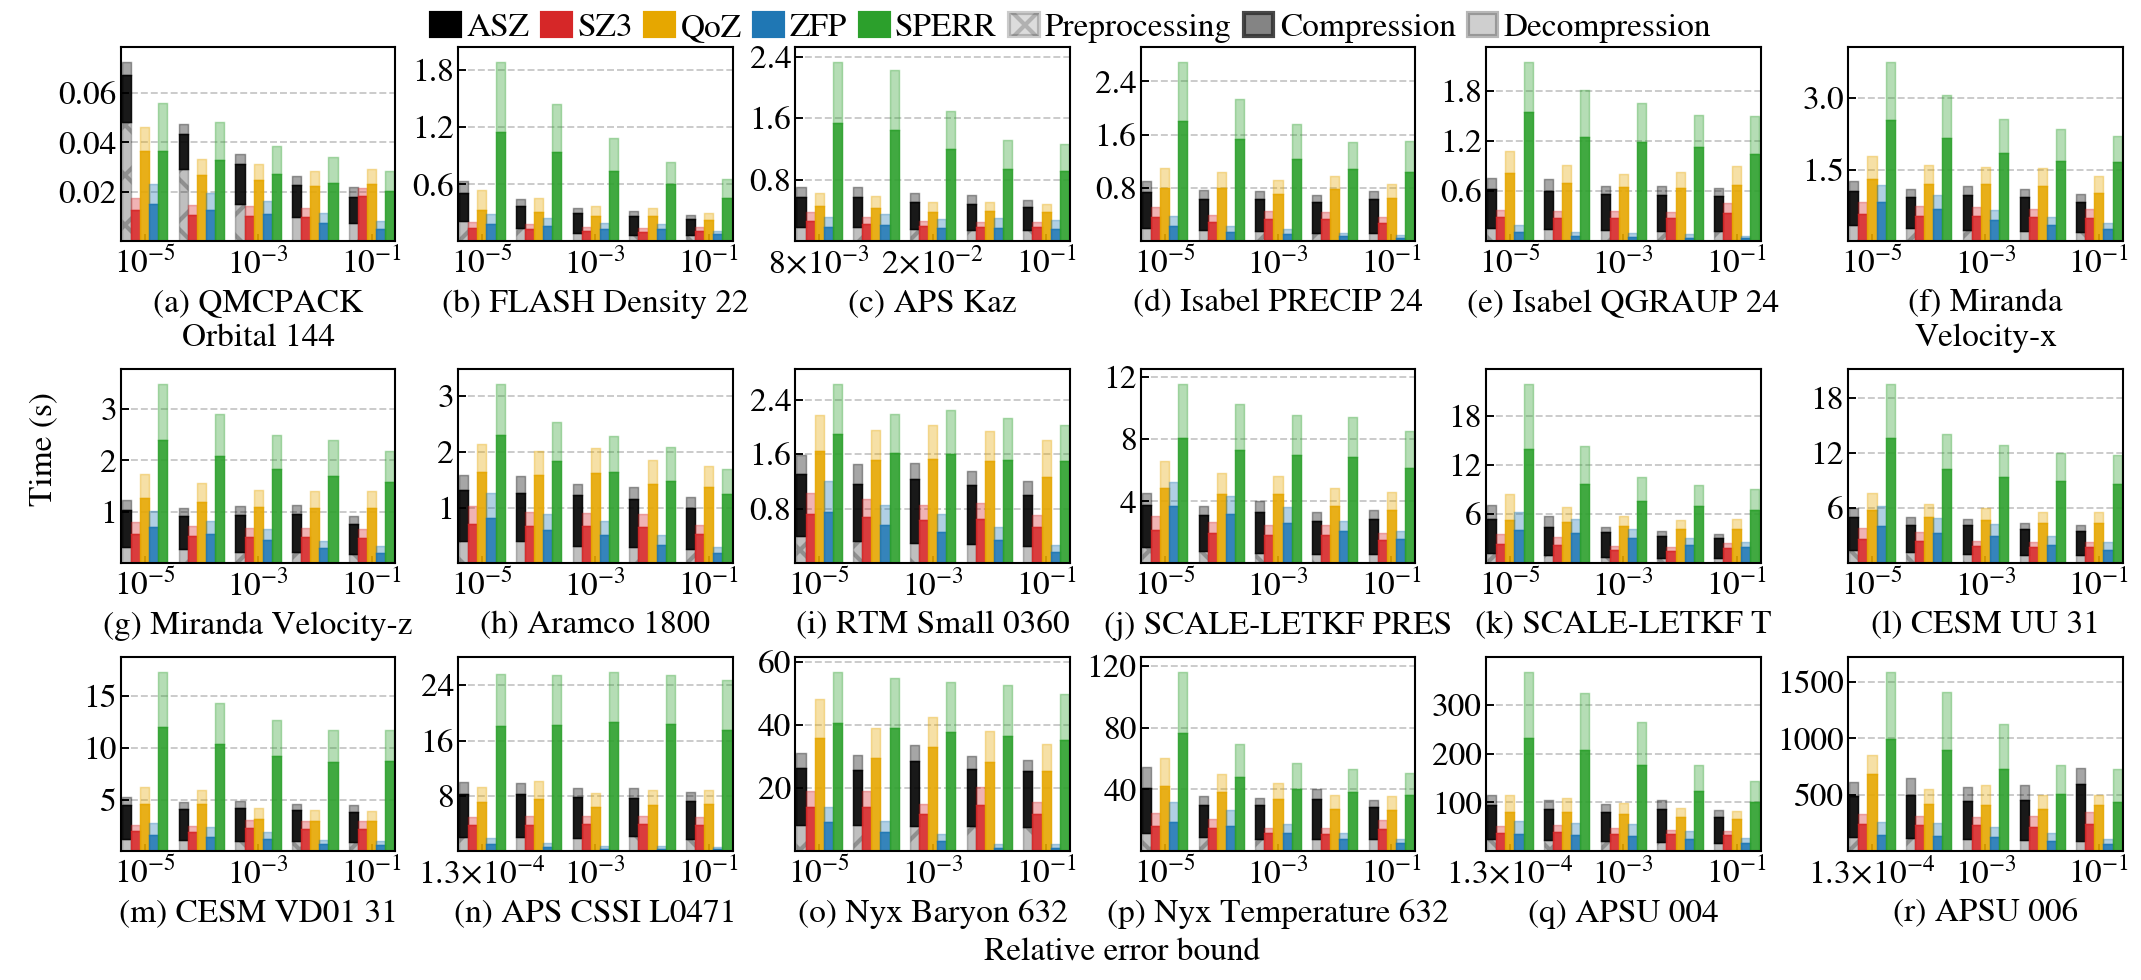
\includegraphics{figs/5/time-breakdown-final-eighteen-vs-rel-eb.png}}{\fbox{\parbox[c][1.5in][c]{0.96\textwidth}{\centering Final 18-field codec-time figure pending.}}}
    \caption{Total runtime across five relative error bounds. Each error-bound group contains one bar per method. ASZ stacks preprocessing, compression, and decompression, while each baseline stacks compression and decompression. ASZ's geometric-mean total runtime is $0.81\times$ that of QoZ and $0.43\times$ that of SPERR.}
    \label{fig:evaluation-codec-time}
\end{figure*}

\subsection{Plan Transferability Across Related Files}
\label{sec:evaluation:transfer}

This subsection evaluates ASZ's ability to reuse a plan generated for one file on other related files. We consider two settings. Temporal reuse shares plans across consecutive snapshots of Isabel PRECIP, RTM Small, and CESM UU. Non-temporal reuse transfers plans across distinct arrays from the same application, namely QMCPACK orbitals, the three Isabel wind components, and two APSU datasets of different sizes.

For an ordered sequence of $T$ files in which $m$ files share one plan, with $m$ odd, we place $\lfloor T/m\rfloor$ contiguous windows of $m$ files at the center of the sequence. The middle file of each window generates the plan for every file in that window. The remaining $T-m\lfloor T/m\rfloor$ files at the two ends lie outside every window and are excluded from the statistics for that $m$, so each target file lies within $(m-1)/2$ positions of the file that generated its plan. Thus, $m=1$ generates a plan for every file, and larger values of $m$ apply each plan to files farther from the file that generated it.

The transferred plan fixes the preprocessing decisions, including each round's prediction axis and QB serialization order. Block coefficients remain adaptive for every target file, as described in Section~\ref{sec:overview:plan-reuse}. Each target file also generates its own plan as the reference, and we compress every file with both plans at relative error bounds $10^{-2}$, $10^{-3}$, and $10^{-4}$. At the PSNR that the self-generated plan attains at $10^{-3}$, we interpolate the bit rate of the transferred plan, $\mathrm{BR}_{\mathrm{transfer}}$, linearly in $\log(\mathrm{BR})$ over PSNR. The relative compression ratio $\mathrm{BR}_{\mathrm{self}}/\mathrm{BR}_{\mathrm{transfer}}$ then compares the two plans at matched PSNR, where $\mathrm{BR}_{\mathrm{self}}$ is the bit rate of the self-generated plan. A value of 1 indicates identical compression ratios, and values below and above 1 indicate that the transferred plan compresses the file worse or better, respectively. For each value of $m$, the average relative compression ratio applies this procedure to the curves averaged over the evaluated files, with BR and normalized mean squared error averaged at each error bound, and the minimum is the smallest value among individual files.

\subsubsection{Temporal Reuse}

The temporal experiment covers Isabel PRECIP time steps 01--48, RTM Small snapshots 0335--0385, and CESM UU time steps 00--62. These sequences contain PRECIP 24, RTM Small 0360, and CESM UU 31 from the 18 evaluated fields. We evaluate $m\in\{1,3,5,9,17\}$.

Figure~\ref{fig:evaluation-temporal-reuse} shows that the average relative compression ratio stays between 0.98 and 1.02 on all three sequences for every $m$. Values above 1 occur because plan generation relies on sampled estimates, so a neighboring file's plan occasionally compresses a target better than the target's own plan. The lowest single-file ratios are 0.87, 0.93, and 0.88 on Isabel PRECIP, RTM Small, and CESM UU, respectively. The minimum varies irregularly with $m$ because it depends on a few files whose windows change with $m$. How many snapshots can share one plan depends on the similarity between snapshots and therefore varies across fields. For the three sequences evaluated here, every group size from 3 to 17 keeps the average compression ratio within 2\% of per-file plan generation.

\begin{figure}[htb]
    \centering
    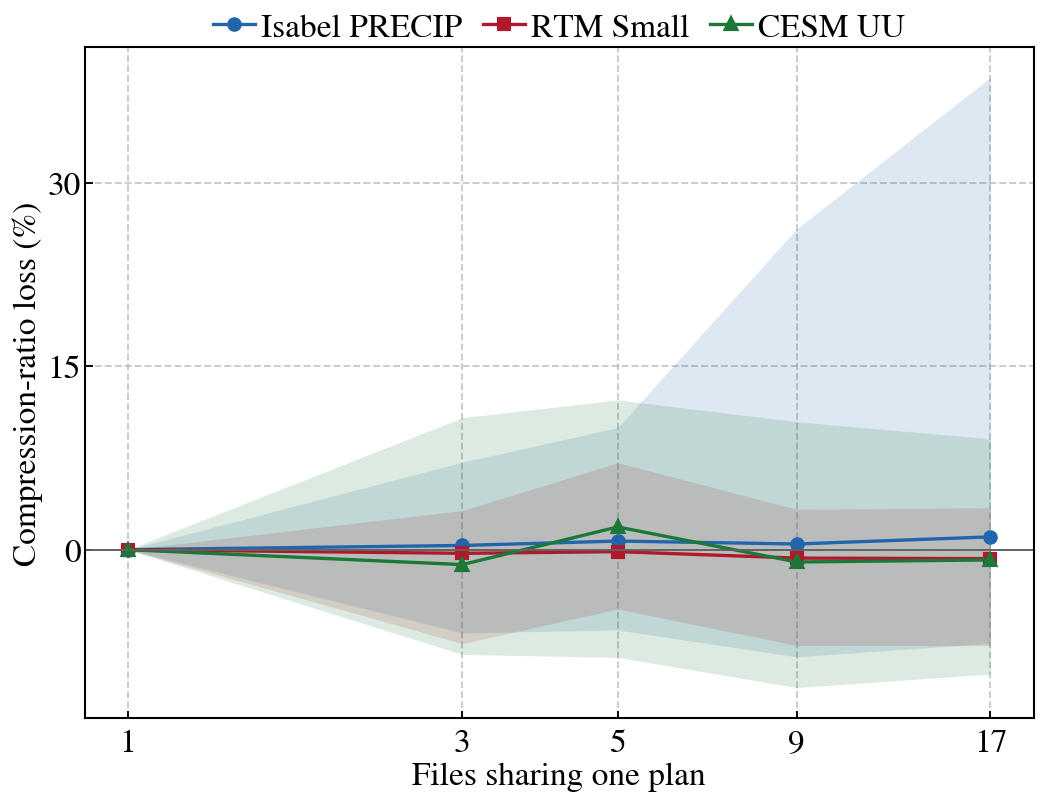
\includegraphics{revised-fig/temporal-plan-reuse.png}
    \caption{Relative compression ratio of temporal plan reuse at matched PSNR. Each panel plots the average over the evaluated files and the minimum over individual files against the number of files that share one plan. A value of 1 means that the transferred plan matches the self-generated plan.}
    \label{fig:evaluation-temporal-reuse}
\end{figure}

\subsubsection{Reuse Across Non-Temporal Related Arrays}

The non-temporal experiments transfer plans across arrays that come from the same application but differ in orbital index, velocity component, or number of frames. Figure~\ref{fig:evaluation-non-temporal-reuse} shows that transferability depends on how similar the arrays are. Neighboring QMCPACK orbitals, the two horizontal Isabel wind components, and the two APSU datasets at fine error bounds exchange plans with little loss, whereas the vertical and horizontal wind components require separate plans.

QMCPACK orbitals 0--287 share the same $115\times69\times69$ spline grid and include QMCPACK orbital 144 from the 18 evaluated fields. We order the orbitals by index and apply the windows defined above with $m\in\{1,3,5,9,17\}$. The average relative compression ratio stays between 0.98 and 0.99 for every $m>1$, but individual orbitals vary more than consecutive snapshots. Six orbitals select 1D4R at $10^{-3}$, and all other orbitals select 1D6R. At $m=3$ and $m=5$, the lowest ratios, 0.63 and 0.67, occur when one of these six orbitals generates the plan for neighbors that select 1D6R. None of these orbitals generates a plan at $m=9$ or $m=17$, and the minimum rises to 0.81 and 0.83, respectively.

Isabel time step 24 provides the wind components U, V, and W on the same $100\times500\times500$ grid, and we apply the plan of each component to the other two. U and V exchange plans with relative compression ratios of 0.99 and 1.00. Plans transferred between W and either horizontal component reach only 0.46 to 0.64. In its two finest rounds, the W plan predicts along the vertical axis, whereas the U and V plans predict along horizontal axes. These two rounds contain about three quarters of all targets, so this difference dominates the compression ratio.

APSU 004 and APSU 006 contain 1024 and 4096 frames, respectively, from the same $1558\times1813$ X-ray detector. We generate the plans on the smaller APSU 004 and apply them to APSU 006, which removes the 102 to 132~s of plan generation on APSU 006. Because this experiment has a single target file, we compute the relative compression ratio at the PSNR of the self-generated plan at each of the five evaluated error bounds. The ratio is at least 0.99 at $10^{-3}$ and finer bounds and decreases to 0.91 at $10^{-2}$ and 0.64 at $10^{-1}$. Plans transferred from the smaller dataset therefore suit APSU 006 from the middle error bound to the finest bound, while the two coarsest bounds benefit from a plan generated on APSU 006 itself.

\begin{figure}[htb]
    \centering
    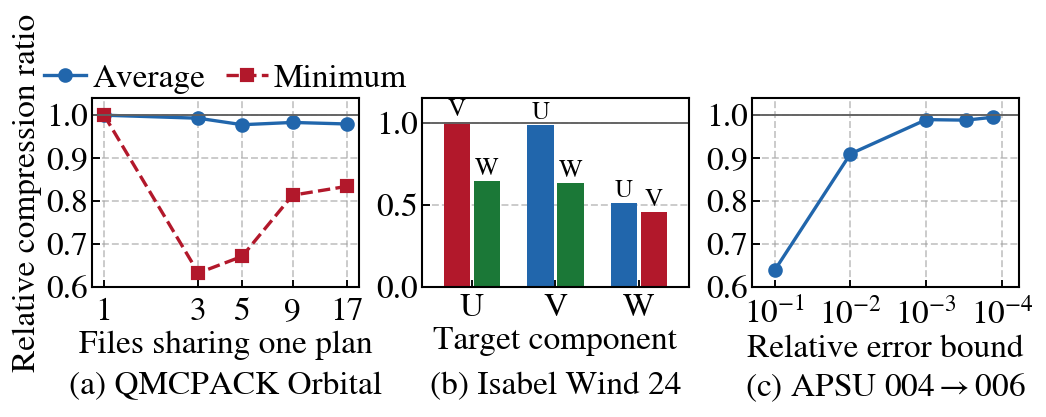
\includegraphics{revised-fig/non-temporal-plan-reuse.png}
    \caption{Relative compression ratio of non-temporal plan reuse at matched PSNR. (a) Average and minimum over QMCPACK orbitals against the number of orbitals that share one plan. (b) Ratio for each Isabel wind component under the plans of the other two components, labeled above each bar. (c) Ratio for APSU 006 under the APSU 004 plan at each error bound. A value of 1 means that the transferred plan matches the self-generated plan.}
    \label{fig:evaluation-non-temporal-reuse}
\end{figure}

\section{Discussion and Limitations}
\label{sec:discussion}

The current design has three main limitations: reverse-greedy search is heuristic, plan reuse targets related arrays from the same application, and the implementation targets three-dimensional interpolation-based compression on CPUs.

Reverse-greedy plan generation fixes each round once and does not guarantee a globally optimal joint configuration. Broader joint or beam search would examine more configurations at additional preprocessing cost.

The transfer experiments cover temporal sequences as well as non-temporal groups of related arrays. Their shared structure comes from one simulation, numerical representation, or acquisition workflow. Each representative is therefore assigned to a compatible group rather than transferred across unrelated applications. Grouping criteria for abrupt phase changes and substantially different tensor structures remain an avenue for future work.

The current implementation and evaluation target single-precision three-dimensional tensors, interpolation-based prediction, and serial CPU execution. Other tensor ranks, predictor classes, and parallel or GPU implementations remain outside the evaluated scope. For an isolated file, preprocessing is part of the measured codec cost. Reuse amortizes this cost only when multiple related files share a plan.

\section{Conclusion}

% TODO: 总结configuration-space reshaping、efficient joint search和实验结果。


\section*{Acknowledgment}
This research was supported by the U.S. Department of Energy, Office of Science, Advanced Scientific Computing Research (ASCR), under contract DE-AC02-06CH11357, and by the National Science Foundation under Grants OAC-2003709, OAC-2104023, OAC-2311875, OAC-2330367, OAC-2311756, and OAC-2313122. We acknowledge the computing resources provided by Bebop at Argonne National Laboratory and the ACCESS Anvil system operated by Purdue University.

\bibliographystyle{IEEEtran}
\bibliography{reference}

\end{document}
